\documentclass[twoside]{book}

% Packages required by doxygen
\usepackage{fixltx2e}
\usepackage{calc}
\usepackage{doxygen}
\usepackage[export]{adjustbox} % also loads graphicx
\usepackage{graphicx}
\usepackage[utf8]{inputenc}
\usepackage{makeidx}
\usepackage{multicol}
\usepackage{multirow}
\PassOptionsToPackage{warn}{textcomp}
\usepackage{textcomp}
\usepackage[nointegrals]{wasysym}
\usepackage[table]{xcolor}

% Font selection
\usepackage[T1]{fontenc}
\usepackage[scaled=.90]{helvet}
\usepackage{courier}
\usepackage{amssymb}
\usepackage{sectsty}
\renewcommand{\familydefault}{\sfdefault}
\allsectionsfont{%
  \fontseries{bc}\selectfont%
  \color{darkgray}%
}
\renewcommand{\DoxyLabelFont}{%
  \fontseries{bc}\selectfont%
  \color{darkgray}%
}
\newcommand{\+}{\discretionary{\mbox{\scriptsize$\hookleftarrow$}}{}{}}

% Page & text layout
\usepackage{geometry}
\geometry{%
  a4paper,%
  top=2.5cm,%
  bottom=2.5cm,%
  left=2.5cm,%
  right=2.5cm%
}
\tolerance=750
\hfuzz=15pt
\hbadness=750
\setlength{\emergencystretch}{15pt}
\setlength{\parindent}{0cm}
\setlength{\parskip}{3ex plus 2ex minus 2ex}
\makeatletter
\renewcommand{\paragraph}{%
  \@startsection{paragraph}{4}{0ex}{-1.0ex}{1.0ex}{%
    \normalfont\normalsize\bfseries\SS@parafont%
  }%
}
\renewcommand{\subparagraph}{%
  \@startsection{subparagraph}{5}{0ex}{-1.0ex}{1.0ex}{%
    \normalfont\normalsize\bfseries\SS@subparafont%
  }%
}
\makeatother

% Headers & footers
\usepackage{fancyhdr}
\pagestyle{fancyplain}
\fancyhead[LE]{\fancyplain{}{\bfseries\thepage}}
\fancyhead[CE]{\fancyplain{}{}}
\fancyhead[RE]{\fancyplain{}{\bfseries\leftmark}}
\fancyhead[LO]{\fancyplain{}{\bfseries\rightmark}}
\fancyhead[CO]{\fancyplain{}{}}
\fancyhead[RO]{\fancyplain{}{\bfseries\thepage}}
\fancyfoot[LE]{\fancyplain{}{}}
\fancyfoot[CE]{\fancyplain{}{}}
\fancyfoot[RE]{\fancyplain{}{\bfseries\scriptsize Generated by Doxygen }}
\fancyfoot[LO]{\fancyplain{}{\bfseries\scriptsize Generated by Doxygen }}
\fancyfoot[CO]{\fancyplain{}{}}
\fancyfoot[RO]{\fancyplain{}{}}
\renewcommand{\footrulewidth}{0.4pt}
\renewcommand{\chaptermark}[1]{%
  \markboth{#1}{}%
}
\renewcommand{\sectionmark}[1]{%
  \markright{\thesection\ #1}%
}

% Indices & bibliography
\usepackage{natbib}
\usepackage[titles]{tocloft}
\setcounter{tocdepth}{3}
\setcounter{secnumdepth}{5}
\makeindex

% Hyperlinks (required, but should be loaded last)
\usepackage{ifpdf}
\ifpdf
  \usepackage[pdftex,pagebackref=true]{hyperref}
\else
  \usepackage[ps2pdf,pagebackref=true]{hyperref}
\fi
\hypersetup{%
  colorlinks=true,%
  linkcolor=blue,%
  citecolor=blue,%
  unicode%
}

% Custom commands
\newcommand{\clearemptydoublepage}{%
  \newpage{\pagestyle{empty}\cleardoublepage}%
}

\usepackage{caption}
\captionsetup{labelsep=space,justification=centering,font={bf},singlelinecheck=off,skip=4pt,position=top}

%===== C O N T E N T S =====

\begin{document}

% Titlepage & ToC
\hypersetup{pageanchor=false,
             bookmarksnumbered=true,
             pdfencoding=unicode
            }
\pagenumbering{alph}
\begin{titlepage}
\vspace*{7cm}
\begin{center}%
{\Large Neat \\[1ex]\large 1.\+0.\+0 }\\
\vspace*{1cm}
{\large Generated by Doxygen 1.8.13}\\
\end{center}
\end{titlepage}
\clearemptydoublepage
\pagenumbering{roman}
\tableofcontents
\clearemptydoublepage
\pagenumbering{arabic}
\hypersetup{pageanchor=true}

%--- Begin generated contents ---
\chapter{Hierarchical Index}
\section{Class Hierarchy}
This inheritance list is sorted roughly, but not completely, alphabetically\+:\begin{DoxyCompactList}
\item \contentsline{section}{Indie\+Neat\+:\+:Backup$<$ num\+Inputs, num\+Outputs $>$}{\pageref{class_indie_neat_1_1_backup}}{}
\item exception\begin{DoxyCompactList}
\item \contentsline{section}{Indie\+Neat\+:\+:Neat\+Engine\+Exception}{\pageref{class_indie_neat_1_1_neat_engine_exception}}{}
\end{DoxyCompactList}
\item \contentsline{section}{Indie\+Neat\+:\+:Genotype$<$ num\+Inputs, num\+Outputs $>$\+:\+:Gene}{\pageref{class_indie_neat_1_1_genotype_1_1_gene}}{}
\item \contentsline{section}{Indie\+Neat\+:\+:Population$<$ num\+Inputs, num\+Outputs $>$\+:\+:Genome\+Container}{\pageref{struct_indie_neat_1_1_population_1_1_genome_container}}{}
\item \contentsline{section}{Indie\+Neat\+:\+:Population$<$ num\+Inputs, num\+Outputs $>$\+:\+:Genome\+Score}{\pageref{struct_indie_neat_1_1_population_1_1_genome_score}}{}
\item \contentsline{section}{Indie\+Neat\+:\+:Genotype$<$ num\+Inputs, num\+Outputs $>$}{\pageref{class_indie_neat_1_1_genotype}}{}
\item \contentsline{section}{Indie\+Neat\+:\+:Mutation\+Manager\+:\+:Mutation}{\pageref{struct_indie_neat_1_1_mutation_manager_1_1_mutation}}{}
\item \contentsline{section}{Indie\+Neat\+:\+:Mutation\+Manager}{\pageref{class_indie_neat_1_1_mutation_manager}}{}
\item \contentsline{section}{Indie\+Neat\+:\+:Mutator$<$ num\+Inputs, num\+Outputs $>$}{\pageref{class_indie_neat_1_1_mutator}}{}
\item \contentsline{section}{Neat\+Engine$<$ num\+Inputs, num\+Outputs $>$}{\pageref{class_neat_engine}}{}
\item \contentsline{section}{Indie\+Neat\+:\+:Neat\+Engine$<$ num\+Inputs, num\+Outputs $>$}{\pageref{class_indie_neat_1_1_neat_engine}}{}
\item \contentsline{section}{Neat\+Pool$<$ T, Args $>$}{\pageref{class_neat_pool}}{}
\item \contentsline{section}{Neat\+Pool$<$ Indie\+Neat\+:\+:Population\+:\+:Species $>$}{\pageref{class_neat_pool}}{}
\item \contentsline{section}{Indie\+Neat\+:\+:Genotype$<$ num\+Inputs, num\+Outputs $>$\+:\+:Node}{\pageref{class_indie_neat_1_1_genotype_1_1_node}}{}
\item \contentsline{section}{Indie\+Neat\+:\+:Operator$<$ num\+Inputs, num\+Outputs $>$}{\pageref{class_indie_neat_1_1_operator}}{}
\item \contentsline{section}{Indie\+Neat\+:\+:Backup$<$ num\+Inputs, num\+Outputs $>$\+:\+:Packed\+Genome}{\pageref{struct_indie_neat_1_1_backup_1_1_packed_genome}}{}
\item \contentsline{section}{Indie\+Neat\+:\+:Backup$<$ num\+Inputs, num\+Outputs $>$\+:\+:Params}{\pageref{struct_indie_neat_1_1_backup_1_1_params}}{}
\item \contentsline{section}{Indie\+Neat\+:\+:Phenotype$<$ num\+Inputs, num\+Outputs $>$}{\pageref{class_indie_neat_1_1_phenotype}}{}
\item \contentsline{section}{Indie\+Neat\+:\+:Population$<$ num\+Inputs, num\+Outputs $>$}{\pageref{class_indie_neat_1_1_population}}{}
\item \contentsline{section}{Indie\+Neat\+:\+:Population$<$ num\+Inputs, num\+Outputs $>$\+:\+:Settings}{\pageref{struct_indie_neat_1_1_population_1_1_settings}}{}
\item \contentsline{section}{Indie\+Neat\+:\+:Operator$<$ num\+Inputs, num\+Outputs $>$\+:\+:Settings}{\pageref{struct_indie_neat_1_1_operator_1_1_settings}}{}
\item \contentsline{section}{Indie\+Neat\+:\+:Mutator$<$ num\+Inputs, num\+Outputs $>$\+:\+:Settings}{\pageref{struct_indie_neat_1_1_mutator_1_1_settings}}{}
\item \contentsline{section}{Indie\+Neat\+:\+:Population$<$ num\+Inputs, num\+Outputs $>$\+:\+:Species}{\pageref{class_indie_neat_1_1_population_1_1_species}}{}
\end{DoxyCompactList}

\chapter{Class Index}
\section{Class List}
Here are the classes, structs, unions and interfaces with brief descriptions\+:\begin{DoxyCompactList}
\item\contentsline{section}{\hyperlink{class_indie_neat_1_1_backup}{Indie\+Neat\+::\+Backup$<$ num\+Inputs, num\+Outputs $>$} }{\pageref{class_indie_neat_1_1_backup}}{}
\item\contentsline{section}{\hyperlink{class_indie_neat_1_1_genotype_1_1_gene}{Indie\+Neat\+::\+Genotype$<$ num\+Inputs, num\+Outputs $>$\+::\+Gene} }{\pageref{class_indie_neat_1_1_genotype_1_1_gene}}{}
\item\contentsline{section}{\hyperlink{struct_indie_neat_1_1_population_1_1_genome_container}{Indie\+Neat\+::\+Population$<$ num\+Inputs, num\+Outputs $>$\+::\+Genome\+Container} }{\pageref{struct_indie_neat_1_1_population_1_1_genome_container}}{}
\item\contentsline{section}{\hyperlink{struct_indie_neat_1_1_population_1_1_genome_score}{Indie\+Neat\+::\+Population$<$ num\+Inputs, num\+Outputs $>$\+::\+Genome\+Score} }{\pageref{struct_indie_neat_1_1_population_1_1_genome_score}}{}
\item\contentsline{section}{\hyperlink{class_indie_neat_1_1_genotype}{Indie\+Neat\+::\+Genotype$<$ num\+Inputs, num\+Outputs $>$} \\*The \hyperlink{class_indie_neat_1_1_genotype}{Genotype} class contains the information about the genome of the artificial neural network }{\pageref{class_indie_neat_1_1_genotype}}{}
\item\contentsline{section}{\hyperlink{struct_indie_neat_1_1_mutation_manager_1_1_mutation}{Indie\+Neat\+::\+Mutation\+Manager\+::\+Mutation} }{\pageref{struct_indie_neat_1_1_mutation_manager_1_1_mutation}}{}
\item\contentsline{section}{\hyperlink{class_indie_neat_1_1_mutation_manager}{Indie\+Neat\+::\+Mutation\+Manager} }{\pageref{class_indie_neat_1_1_mutation_manager}}{}
\item\contentsline{section}{\hyperlink{class_indie_neat_1_1_mutator}{Indie\+Neat\+::\+Mutator$<$ num\+Inputs, num\+Outputs $>$} }{\pageref{class_indie_neat_1_1_mutator}}{}
\item\contentsline{section}{\hyperlink{class_neat_engine}{Neat\+Engine$<$ num\+Inputs, num\+Outputs $>$} }{\pageref{class_neat_engine}}{}
\item\contentsline{section}{\hyperlink{class_indie_neat_1_1_neat_engine}{Indie\+Neat\+::\+Neat\+Engine$<$ num\+Inputs, num\+Outputs $>$} }{\pageref{class_indie_neat_1_1_neat_engine}}{}
\item\contentsline{section}{\hyperlink{class_indie_neat_1_1_neat_engine_exception}{Indie\+Neat\+::\+Neat\+Engine\+Exception} }{\pageref{class_indie_neat_1_1_neat_engine_exception}}{}
\item\contentsline{section}{\hyperlink{class_neat_pool}{Neat\+Pool$<$ T, Args $>$} }{\pageref{class_neat_pool}}{}
\item\contentsline{section}{\hyperlink{class_indie_neat_1_1_genotype_1_1_node}{Indie\+Neat\+::\+Genotype$<$ num\+Inputs, num\+Outputs $>$\+::\+Node} }{\pageref{class_indie_neat_1_1_genotype_1_1_node}}{}
\item\contentsline{section}{\hyperlink{class_indie_neat_1_1_operator}{Indie\+Neat\+::\+Operator$<$ num\+Inputs, num\+Outputs $>$} }{\pageref{class_indie_neat_1_1_operator}}{}
\item\contentsline{section}{\hyperlink{struct_indie_neat_1_1_backup_1_1_packed_genome}{Indie\+Neat\+::\+Backup$<$ num\+Inputs, num\+Outputs $>$\+::\+Packed\+Genome} }{\pageref{struct_indie_neat_1_1_backup_1_1_packed_genome}}{}
\item\contentsline{section}{\hyperlink{struct_indie_neat_1_1_backup_1_1_params}{Indie\+Neat\+::\+Backup$<$ num\+Inputs, num\+Outputs $>$\+::\+Params} }{\pageref{struct_indie_neat_1_1_backup_1_1_params}}{}
\item\contentsline{section}{\hyperlink{class_indie_neat_1_1_phenotype}{Indie\+Neat\+::\+Phenotype$<$ num\+Inputs, num\+Outputs $>$} \\*Allows to interpret \hyperlink{class_indie_neat_1_1_genotype}{Genotype} into \hyperlink{class_indie_neat_1_1_phenotype}{Phenotype} }{\pageref{class_indie_neat_1_1_phenotype}}{}
\item\contentsline{section}{\hyperlink{class_indie_neat_1_1_population}{Indie\+Neat\+::\+Population$<$ num\+Inputs, num\+Outputs $>$} }{\pageref{class_indie_neat_1_1_population}}{}
\item\contentsline{section}{\hyperlink{struct_indie_neat_1_1_population_1_1_settings}{Indie\+Neat\+::\+Population$<$ num\+Inputs, num\+Outputs $>$\+::\+Settings} }{\pageref{struct_indie_neat_1_1_population_1_1_settings}}{}
\item\contentsline{section}{\hyperlink{struct_indie_neat_1_1_operator_1_1_settings}{Indie\+Neat\+::\+Operator$<$ num\+Inputs, num\+Outputs $>$\+::\+Settings} }{\pageref{struct_indie_neat_1_1_operator_1_1_settings}}{}
\item\contentsline{section}{\hyperlink{struct_indie_neat_1_1_mutator_1_1_settings}{Indie\+Neat\+::\+Mutator$<$ num\+Inputs, num\+Outputs $>$\+::\+Settings} }{\pageref{struct_indie_neat_1_1_mutator_1_1_settings}}{}
\item\contentsline{section}{\hyperlink{class_indie_neat_1_1_population_1_1_species}{Indie\+Neat\+::\+Population$<$ num\+Inputs, num\+Outputs $>$\+::\+Species} }{\pageref{class_indie_neat_1_1_population_1_1_species}}{}
\end{DoxyCompactList}

\chapter{Class Documentation}
\hypertarget{class_indie_neat_1_1_backup}{}\section{Indie\+Neat\+:\+:Backup$<$ num\+Inputs, num\+Outputs $>$ Class Template Reference}
\label{class_indie_neat_1_1_backup}\index{Indie\+Neat\+::\+Backup$<$ num\+Inputs, num\+Outputs $>$@{Indie\+Neat\+::\+Backup$<$ num\+Inputs, num\+Outputs $>$}}
\subsection*{Classes}
\begin{DoxyCompactItemize}
\item 
struct \hyperlink{struct_indie_neat_1_1_backup_1_1_packed_genome}{Packed\+Genome}
\item 
struct \hyperlink{struct_indie_neat_1_1_backup_1_1_params}{Params}
\end{DoxyCompactItemize}
\subsection*{Static Public Member Functions}
\begin{DoxyCompactItemize}
\item 
\mbox{\Hypertarget{class_indie_neat_1_1_backup_a773e9e13579a40543ca31ceac3c21ba2}\label{class_indie_neat_1_1_backup_a773e9e13579a40543ca31ceac3c21ba2}} 
static bool {\bfseries save\+Params} (\hyperlink{class_indie_neat_1_1_neat_engine}{Neat\+Engine}$<$ num\+Inputs, num\+Outputs $>$ const \&engine)
\item 
\mbox{\Hypertarget{class_indie_neat_1_1_backup_a2b8db0837a930e491f692c7b9fccbccd}\label{class_indie_neat_1_1_backup_a2b8db0837a930e491f692c7b9fccbccd}} 
static void {\bfseries encode\+Genome} (\hyperlink{class_indie_neat_1_1_genotype}{Genotype}$<$ num\+Inputs, num\+Outputs $>$ \&genome, std\+::string \&saver)
\item 
\mbox{\Hypertarget{class_indie_neat_1_1_backup_aacb848f2c3955f1c6354a5153efe224b}\label{class_indie_neat_1_1_backup_aacb848f2c3955f1c6354a5153efe224b}} 
static bool {\bfseries encode\+Genome} (\hyperlink{class_indie_neat_1_1_genotype}{Genotype}$<$ num\+Inputs, num\+Outputs $>$ \&genome, std\+::string const \&filename)
\item 
\mbox{\Hypertarget{class_indie_neat_1_1_backup_ac58b81e59e3781d9eb1c3d408380c6db}\label{class_indie_neat_1_1_backup_ac58b81e59e3781d9eb1c3d408380c6db}} 
static bool {\bfseries decode\+Genome} (\hyperlink{struct_indie_neat_1_1_backup_1_1_packed_genome}{Packed\+Genome} \&genome, std\+::string const \&filename)
\item 
\mbox{\Hypertarget{class_indie_neat_1_1_backup_a817b72045a454b966f9a4a45d5a61e31}\label{class_indie_neat_1_1_backup_a817b72045a454b966f9a4a45d5a61e31}} 
static std\+::string const  \& {\bfseries get\+Directory} ()
\item 
\mbox{\Hypertarget{class_indie_neat_1_1_backup_ab30a6d7996f11c8a13bc1c9489a10e29}\label{class_indie_neat_1_1_backup_ab30a6d7996f11c8a13bc1c9489a10e29}} 
static bool {\bfseries set\+Directory} (std\+::string const \&dir)
\item 
\mbox{\Hypertarget{class_indie_neat_1_1_backup_a3a6daec23ae5c450d66da35bd13e3c6f}\label{class_indie_neat_1_1_backup_a3a6daec23ae5c450d66da35bd13e3c6f}} 
static bool {\bfseries get\+Params} (\hyperlink{struct_indie_neat_1_1_backup_1_1_params}{Params} \&params)
\end{DoxyCompactItemize}


The documentation for this class was generated from the following file\+:\begin{DoxyCompactItemize}
\item 
src/Backup.\+hpp\end{DoxyCompactItemize}

\hypertarget{class_indie_neat_1_1_genotype_1_1_gene}{}\section{Indie\+Neat\+:\+:Genotype$<$ num\+Inputs, num\+Outputs $>$\+:\+:Gene Class Reference}
\label{class_indie_neat_1_1_genotype_1_1_gene}\index{Indie\+Neat\+::\+Genotype$<$ num\+Inputs, num\+Outputs $>$\+::\+Gene@{Indie\+Neat\+::\+Genotype$<$ num\+Inputs, num\+Outputs $>$\+::\+Gene}}


{\ttfamily \#include $<$Genotype.\+hpp$>$}

\subsection*{Public Member Functions}
\begin{DoxyCompactItemize}
\item 
\mbox{\Hypertarget{class_indie_neat_1_1_genotype_1_1_gene_a71a4944914ec3297e96f576fb7e71dae}\label{class_indie_neat_1_1_genotype_1_1_gene_a71a4944914ec3297e96f576fb7e71dae}} 
{\bfseries Gene} (unsigned int input, unsigned int output, long long innov, std\+::pair$<$ double, double $>$ const \&range)
\item 
\mbox{\Hypertarget{class_indie_neat_1_1_genotype_1_1_gene_a1b1f01785939b796e2618404d25382cd}\label{class_indie_neat_1_1_genotype_1_1_gene_a1b1f01785939b796e2618404d25382cd}} 
{\bfseries Gene} (unsigned int input, unsigned int output, long long innov, bool enabled, double weight)
\item 
\mbox{\Hypertarget{class_indie_neat_1_1_genotype_1_1_gene_a94196bcc044ed7e9c3ac9372fe51a95e}\label{class_indie_neat_1_1_genotype_1_1_gene_a94196bcc044ed7e9c3ac9372fe51a95e}} 
{\bfseries Gene} (\hyperlink{class_indie_neat_1_1_genotype_1_1_gene}{Gene} const \&copy)
\item 
\mbox{\Hypertarget{class_indie_neat_1_1_genotype_1_1_gene_a10bf052f60f2fc95748db1ce1d45a839}\label{class_indie_neat_1_1_genotype_1_1_gene_a10bf052f60f2fc95748db1ce1d45a839}} 
\hyperlink{class_indie_neat_1_1_genotype_1_1_gene}{Gene} \& {\bfseries operator=} (\hyperlink{class_indie_neat_1_1_genotype_1_1_gene}{Gene} const \&copy)
\item 
\mbox{\Hypertarget{class_indie_neat_1_1_genotype_1_1_gene_a10816dbb01b1612f72ee896a365dc64d}\label{class_indie_neat_1_1_genotype_1_1_gene_a10816dbb01b1612f72ee896a365dc64d}} 
void {\bfseries set\+Weight} (double weight)
\item 
\mbox{\Hypertarget{class_indie_neat_1_1_genotype_1_1_gene_a21d12992bf1aaeac620d6080365f4b65}\label{class_indie_neat_1_1_genotype_1_1_gene_a21d12992bf1aaeac620d6080365f4b65}} 
double {\bfseries get\+Weight} (void) const
\item 
\mbox{\Hypertarget{class_indie_neat_1_1_genotype_1_1_gene_ae6c7def704522367a17e24f0b5d34a2d}\label{class_indie_neat_1_1_genotype_1_1_gene_ae6c7def704522367a17e24f0b5d34a2d}} 
void {\bfseries toggle\+Enabled} (void)
\item 
\mbox{\Hypertarget{class_indie_neat_1_1_genotype_1_1_gene_ace348052be7366d9617f300e04432f6a}\label{class_indie_neat_1_1_genotype_1_1_gene_ace348052be7366d9617f300e04432f6a}} 
void {\bfseries set\+Enabled} (bool enabled)
\item 
\mbox{\Hypertarget{class_indie_neat_1_1_genotype_1_1_gene_a0500752fe9bccddb2e75b8624bb970fb}\label{class_indie_neat_1_1_genotype_1_1_gene_a0500752fe9bccddb2e75b8624bb970fb}} 
bool {\bfseries is\+Enabled} (void) const
\item 
\mbox{\Hypertarget{class_indie_neat_1_1_genotype_1_1_gene_a1bc8e6ee64605d55297b4e2be10750bd}\label{class_indie_neat_1_1_genotype_1_1_gene_a1bc8e6ee64605d55297b4e2be10750bd}} 
long long {\bfseries get\+Ino} (void) const
\item 
\mbox{\Hypertarget{class_indie_neat_1_1_genotype_1_1_gene_af2ada5b6314d0af72535a1770e4d20f1}\label{class_indie_neat_1_1_genotype_1_1_gene_af2ada5b6314d0af72535a1770e4d20f1}} 
unsigned int {\bfseries Input} (void) const
\item 
\mbox{\Hypertarget{class_indie_neat_1_1_genotype_1_1_gene_a8533d25d547d637ca4ca78cba2c90aed}\label{class_indie_neat_1_1_genotype_1_1_gene_a8533d25d547d637ca4ca78cba2c90aed}} 
unsigned int {\bfseries Output} (void) const
\end{DoxyCompactItemize}


\subsection{Detailed Description}
\subsubsection*{template$<$unsigned int num\+Inputs, unsigned int num\+Outputs$>$\newline
class Indie\+Neat\+::\+Genotype$<$ num\+Inputs, num\+Outputs $>$\+::\+Gene}

The class \hyperlink{class_indie_neat_1_1_genotype_1_1_gene}{Gene} contains all the information about a gene in the genome. With this class we can know where the gene is, between which \hyperlink{class_indie_neat_1_1_genotype_1_1_node}{Node}. We also know its innovation number, which is the rank of the gene creation. Finally, we have the current coefficient of the gene, which is the knowledge contained inside it. 

The documentation for this class was generated from the following file\+:\begin{DoxyCompactItemize}
\item 
src/Genotype.\+hpp\end{DoxyCompactItemize}

\hypertarget{struct_indie_neat_1_1_population_1_1_genome_container}{}\section{Indie\+Neat\+:\+:Population$<$ num\+Inputs, num\+Outputs $>$\+:\+:Genome\+Container Struct Reference}
\label{struct_indie_neat_1_1_population_1_1_genome_container}\index{Indie\+Neat\+::\+Population$<$ num\+Inputs, num\+Outputs $>$\+::\+Genome\+Container@{Indie\+Neat\+::\+Population$<$ num\+Inputs, num\+Outputs $>$\+::\+Genome\+Container}}
\subsection*{Public Member Functions}
\begin{DoxyCompactItemize}
\item 
\mbox{\Hypertarget{struct_indie_neat_1_1_population_1_1_genome_container_a85a60321b3d308c05b0bdb15ecff6e06}\label{struct_indie_neat_1_1_population_1_1_genome_container_a85a60321b3d308c05b0bdb15ecff6e06}} 
{\bfseries Genome\+Container} (unsigned int id, \hyperlink{class_indie_neat_1_1_genotype}{Genotype}$<$ num\+Inputs, num\+Outputs $>$ \&g)
\item 
\mbox{\Hypertarget{struct_indie_neat_1_1_population_1_1_genome_container_a1da0baf8fba962d13db18d200ea7f1a1}\label{struct_indie_neat_1_1_population_1_1_genome_container_a1da0baf8fba962d13db18d200ea7f1a1}} 
{\bfseries Genome\+Container} (\hyperlink{struct_indie_neat_1_1_population_1_1_genome_container}{Genome\+Container} const \&copy)
\item 
\mbox{\Hypertarget{struct_indie_neat_1_1_population_1_1_genome_container_aa9a6435f66f80cfda0169b07235b8821}\label{struct_indie_neat_1_1_population_1_1_genome_container_aa9a6435f66f80cfda0169b07235b8821}} 
\hyperlink{struct_indie_neat_1_1_population_1_1_genome_container}{Genome\+Container} \& {\bfseries operator=} (\hyperlink{struct_indie_neat_1_1_population_1_1_genome_container}{Genome\+Container} const \&copy)
\end{DoxyCompactItemize}
\subsection*{Public Attributes}
\begin{DoxyCompactItemize}
\item 
\mbox{\Hypertarget{struct_indie_neat_1_1_population_1_1_genome_container_ac2a981c2c2e2737408fa51e586642883}\label{struct_indie_neat_1_1_population_1_1_genome_container_ac2a981c2c2e2737408fa51e586642883}} 
unsigned int {\bfseries idx}
\item 
\mbox{\Hypertarget{struct_indie_neat_1_1_population_1_1_genome_container_a4ec95dc29ab8fa7544fdbb664f027dcc}\label{struct_indie_neat_1_1_population_1_1_genome_container_a4ec95dc29ab8fa7544fdbb664f027dcc}} 
\hyperlink{class_indie_neat_1_1_genotype}{Genotype}$<$ num\+Inputs, num\+Outputs $>$ $\ast$ {\bfseries genome}
\end{DoxyCompactItemize}


The documentation for this struct was generated from the following file\+:\begin{DoxyCompactItemize}
\item 
src/Population.\+hpp\end{DoxyCompactItemize}

\hypertarget{struct_indie_neat_1_1_population_1_1_genome_score}{}\section{Indie\+Neat\+:\+:Population$<$ num\+Inputs, num\+Outputs $>$\+:\+:Genome\+Score Struct Reference}
\label{struct_indie_neat_1_1_population_1_1_genome_score}\index{Indie\+Neat\+::\+Population$<$ num\+Inputs, num\+Outputs $>$\+::\+Genome\+Score@{Indie\+Neat\+::\+Population$<$ num\+Inputs, num\+Outputs $>$\+::\+Genome\+Score}}
\subsection*{Public Member Functions}
\begin{DoxyCompactItemize}
\item 
\mbox{\Hypertarget{struct_indie_neat_1_1_population_1_1_genome_score_a21fa32aada642143ca766d25da3d1243}\label{struct_indie_neat_1_1_population_1_1_genome_score_a21fa32aada642143ca766d25da3d1243}} 
{\bfseries Genome\+Score} (unsigned int id, double f)
\item 
\mbox{\Hypertarget{struct_indie_neat_1_1_population_1_1_genome_score_a069cd75c33671ba8dcb95339e81208c6}\label{struct_indie_neat_1_1_population_1_1_genome_score_a069cd75c33671ba8dcb95339e81208c6}} 
{\bfseries Genome\+Score} (\hyperlink{struct_indie_neat_1_1_population_1_1_genome_score}{Genome\+Score} const \&copy)
\item 
\mbox{\Hypertarget{struct_indie_neat_1_1_population_1_1_genome_score_ab505cea6c6acfd9f0631a8c8ecfdd2f5}\label{struct_indie_neat_1_1_population_1_1_genome_score_ab505cea6c6acfd9f0631a8c8ecfdd2f5}} 
\hyperlink{struct_indie_neat_1_1_population_1_1_genome_score}{Genome\+Score} \& {\bfseries operator=} (\hyperlink{struct_indie_neat_1_1_population_1_1_genome_score}{Genome\+Score} const \&copy)
\end{DoxyCompactItemize}
\subsection*{Public Attributes}
\begin{DoxyCompactItemize}
\item 
\mbox{\Hypertarget{struct_indie_neat_1_1_population_1_1_genome_score_ad270cdeb2ae09bf2c456d2b220731535}\label{struct_indie_neat_1_1_population_1_1_genome_score_ad270cdeb2ae09bf2c456d2b220731535}} 
unsigned int {\bfseries idx}
\item 
\mbox{\Hypertarget{struct_indie_neat_1_1_population_1_1_genome_score_a060d718f8c10ad1f20d9cadbe7170d52}\label{struct_indie_neat_1_1_population_1_1_genome_score_a060d718f8c10ad1f20d9cadbe7170d52}} 
double {\bfseries fitness}
\end{DoxyCompactItemize}


The documentation for this struct was generated from the following file\+:\begin{DoxyCompactItemize}
\item 
src/Population.\+hpp\end{DoxyCompactItemize}

\hypertarget{class_indie_neat_1_1_genotype}{}\section{Indie\+Neat\+:\+:Genotype$<$ num\+Inputs, num\+Outputs $>$ Class Template Reference}
\label{class_indie_neat_1_1_genotype}\index{Indie\+Neat\+::\+Genotype$<$ num\+Inputs, num\+Outputs $>$@{Indie\+Neat\+::\+Genotype$<$ num\+Inputs, num\+Outputs $>$}}


The \hyperlink{class_indie_neat_1_1_genotype}{Genotype} class contains the information about the genome of the artificial neural network.  




{\ttfamily \#include $<$Genotype.\+hpp$>$}

\subsection*{Classes}
\begin{DoxyCompactItemize}
\item 
class \hyperlink{class_indie_neat_1_1_genotype_1_1_gene}{Gene}
\item 
class \hyperlink{class_indie_neat_1_1_genotype_1_1_node}{Node}
\end{DoxyCompactItemize}
\subsection*{Public Types}
\begin{DoxyCompactItemize}
\item 
\mbox{\Hypertarget{class_indie_neat_1_1_genotype_a3c565c5d61ead686f245d585ddfa2507}\label{class_indie_neat_1_1_genotype_a3c565c5d61ead686f245d585ddfa2507}} 
enum {\bfseries Node\+Type} \{ {\bfseries I\+N\+P\+UT}, 
{\bfseries O\+U\+T\+P\+UT}, 
{\bfseries H\+I\+D\+D\+EN}
 \}
\item 
\mbox{\Hypertarget{class_indie_neat_1_1_genotype_a2e76da677f35a309198db3465cbf6561}\label{class_indie_neat_1_1_genotype_a2e76da677f35a309198db3465cbf6561}} 
enum {\bfseries State} \{ {\bfseries N\+O\+T\+\_\+\+E\+V\+A\+L\+U\+A\+T\+ED}, 
{\bfseries I\+N\+\_\+\+E\+V\+A\+L\+U\+A\+T\+I\+ON}, 
{\bfseries I\+S\+\_\+\+E\+V\+A\+L\+U\+A\+T\+ED}
 \}
\end{DoxyCompactItemize}
\subsection*{Public Member Functions}
\begin{DoxyCompactItemize}
\item 
\mbox{\Hypertarget{class_indie_neat_1_1_genotype_ae0580322e5095a549a514af6986e92ae}\label{class_indie_neat_1_1_genotype_ae0580322e5095a549a514af6986e92ae}} 
{\bfseries Genotype} (std\+::pair$<$ double, double $>$ const \&range)
\item 
\mbox{\Hypertarget{class_indie_neat_1_1_genotype_a61b75e0ad6ab03232cda13ab7de78c79}\label{class_indie_neat_1_1_genotype_a61b75e0ad6ab03232cda13ab7de78c79}} 
{\bfseries Genotype} (\hyperlink{class_indie_neat_1_1_genotype}{Genotype} const \&copy)
\item 
\mbox{\Hypertarget{class_indie_neat_1_1_genotype_afaac0a604631f5d52c5a3d2d9ba737b3}\label{class_indie_neat_1_1_genotype_afaac0a604631f5d52c5a3d2d9ba737b3}} 
\hyperlink{class_indie_neat_1_1_genotype}{Genotype} \& {\bfseries operator=} (\hyperlink{class_indie_neat_1_1_genotype}{Genotype} const \&copy)
\item 
\mbox{\Hypertarget{class_indie_neat_1_1_genotype_a660be7d08066d8a4d4dbd98fc90d9e64}\label{class_indie_neat_1_1_genotype_a660be7d08066d8a4d4dbd98fc90d9e64}} 
std\+::vector$<$ \hyperlink{class_indie_neat_1_1_genotype_1_1_node}{Node} $\ast$ $>$ \& {\bfseries Nodes} (void)
\item 
\mbox{\Hypertarget{class_indie_neat_1_1_genotype_a5e07223bea57cce159a4856b0f1d4be9}\label{class_indie_neat_1_1_genotype_a5e07223bea57cce159a4856b0f1d4be9}} 
std\+::vector$<$ \hyperlink{class_indie_neat_1_1_genotype_1_1_gene}{Gene} $\ast$ $>$ \& {\bfseries Genes} (void)
\item 
\mbox{\Hypertarget{class_indie_neat_1_1_genotype_a21689d356b3e334dcc748b303537a7c5}\label{class_indie_neat_1_1_genotype_a21689d356b3e334dcc748b303537a7c5}} 
std\+::vector$<$ \hyperlink{class_indie_neat_1_1_genotype_1_1_node}{Node} $\ast$ $>$ const  \& {\bfseries Nodes} (void) const
\item 
\mbox{\Hypertarget{class_indie_neat_1_1_genotype_a27509878844ce83fde93f94c62f031b9}\label{class_indie_neat_1_1_genotype_a27509878844ce83fde93f94c62f031b9}} 
std\+::vector$<$ \hyperlink{class_indie_neat_1_1_genotype_1_1_gene}{Gene} $\ast$ $>$ const  \& {\bfseries Genes} (void) const
\item 
\mbox{\Hypertarget{class_indie_neat_1_1_genotype_a177c51e16af584e32f33aa0b2274f6b0}\label{class_indie_neat_1_1_genotype_a177c51e16af584e32f33aa0b2274f6b0}} 
void {\bfseries get\+Inputs} (std\+::vector$<$ unsigned int $>$ \&inputs) const
\item 
\mbox{\Hypertarget{class_indie_neat_1_1_genotype_afd23aecb452ee3377e3da9c225db2cbf}\label{class_indie_neat_1_1_genotype_afd23aecb452ee3377e3da9c225db2cbf}} 
void {\bfseries get\+Outputs} (std\+::vector$<$ unsigned int $>$ \&outputs) const
\item 
\mbox{\Hypertarget{class_indie_neat_1_1_genotype_a591f9866b698b3c3e687298e1edaa5e9}\label{class_indie_neat_1_1_genotype_a591f9866b698b3c3e687298e1edaa5e9}} 
\hyperlink{class_indie_neat_1_1_genotype_1_1_node}{Node} $\ast$ {\bfseries add\+Node} (Node\+Type type, std\+::pair$<$ double, double $>$ const \&range)
\item 
\mbox{\Hypertarget{class_indie_neat_1_1_genotype_a61c94ac7533eadc6c710522a5e577977}\label{class_indie_neat_1_1_genotype_a61c94ac7533eadc6c710522a5e577977}} 
void {\bfseries set\+Fitness} (double fitness)
\item 
\mbox{\Hypertarget{class_indie_neat_1_1_genotype_a79a07d4c8ab04900d1630aa86d6eba76}\label{class_indie_neat_1_1_genotype_a79a07d4c8ab04900d1630aa86d6eba76}} 
double {\bfseries get\+Fitness} (void) const
\item 
\mbox{\Hypertarget{class_indie_neat_1_1_genotype_a371bdcc52d4ac1ba306354413a772df4}\label{class_indie_neat_1_1_genotype_a371bdcc52d4ac1ba306354413a772df4}} 
void {\bfseries set\+State} (State state)
\item 
\mbox{\Hypertarget{class_indie_neat_1_1_genotype_ab5b6bbab4dbed77350d30a051ab621e7}\label{class_indie_neat_1_1_genotype_ab5b6bbab4dbed77350d30a051ab621e7}} 
State {\bfseries get\+State} (void) const
\item 
\mbox{\Hypertarget{class_indie_neat_1_1_genotype_a3962be224016a1646612027fb1ecf578}\label{class_indie_neat_1_1_genotype_a3962be224016a1646612027fb1ecf578}} 
long long {\bfseries get\+Num\+Nodes} (void) const
\item 
\mbox{\Hypertarget{class_indie_neat_1_1_genotype_a7d0ab4939bfe9eef825e7ab5065d1780}\label{class_indie_neat_1_1_genotype_a7d0ab4939bfe9eef825e7ab5065d1780}} 
void {\bfseries set\+Num\+Nodes} (long long num)
\end{DoxyCompactItemize}


\subsection{Detailed Description}
\subsubsection*{template$<$unsigned int num\+Inputs, unsigned int num\+Outputs$>$\newline
class Indie\+Neat\+::\+Genotype$<$ num\+Inputs, num\+Outputs $>$}

The \hyperlink{class_indie_neat_1_1_genotype}{Genotype} class contains the information about the genome of the artificial neural network. 

Inside the \hyperlink{class_indie_neat_1_1_genotype}{Genotype} class we can retrieve each \hyperlink{class_indie_neat_1_1_genotype_1_1_node}{Node} and each \hyperlink{class_indie_neat_1_1_genotype_1_1_gene}{Gene} which contains all the knowledge of the artificial neural network. We can also retrieve all the path in the evolution history of the artificial neural network population. 
\begin{DoxyTemplParams}{Template Parameters}
{\em num\+Inputs} & Contains how many inputs has the genotype. \\
\hline
{\em num\+Outputs} & Contains how many outputs has the genotype. \\
\hline
\end{DoxyTemplParams}


The documentation for this class was generated from the following file\+:\begin{DoxyCompactItemize}
\item 
src/Genotype.\+hpp\end{DoxyCompactItemize}

\hypertarget{struct_indie_neat_1_1_mutation_manager_1_1_mutation}{}\section{Indie\+Neat\+:\+:Mutation\+Manager\+:\+:Mutation Struct Reference}
\label{struct_indie_neat_1_1_mutation_manager_1_1_mutation}\index{Indie\+Neat\+::\+Mutation\+Manager\+::\+Mutation@{Indie\+Neat\+::\+Mutation\+Manager\+::\+Mutation}}
\subsection*{Public Attributes}
\begin{DoxyCompactItemize}
\item 
\mbox{\Hypertarget{struct_indie_neat_1_1_mutation_manager_1_1_mutation_a0a1d87a46b4496068a605d4a90642416}\label{struct_indie_neat_1_1_mutation_manager_1_1_mutation_a0a1d87a46b4496068a605d4a90642416}} 
unsigned int {\bfseries input}
\item 
\mbox{\Hypertarget{struct_indie_neat_1_1_mutation_manager_1_1_mutation_aeaf66cca2fd67b42eed52dc19e6ec0bb}\label{struct_indie_neat_1_1_mutation_manager_1_1_mutation_aeaf66cca2fd67b42eed52dc19e6ec0bb}} 
unsigned int {\bfseries output}
\item 
\mbox{\Hypertarget{struct_indie_neat_1_1_mutation_manager_1_1_mutation_a651ca54d21cc4859ee42349eedd9fafe}\label{struct_indie_neat_1_1_mutation_manager_1_1_mutation_a651ca54d21cc4859ee42349eedd9fafe}} 
Mutation\+Type {\bfseries type}
\item 
\mbox{\Hypertarget{struct_indie_neat_1_1_mutation_manager_1_1_mutation_aac7f68b32f823fbe57ee270e89397ab6}\label{struct_indie_neat_1_1_mutation_manager_1_1_mutation_aac7f68b32f823fbe57ee270e89397ab6}} 
long long {\bfseries innov}
\end{DoxyCompactItemize}


The documentation for this struct was generated from the following file\+:\begin{DoxyCompactItemize}
\item 
src/Mutation\+Manager.\+hh\end{DoxyCompactItemize}

\hypertarget{class_indie_neat_1_1_mutation_manager}{}\section{Indie\+Neat\+:\+:Mutation\+Manager Class Reference}
\label{class_indie_neat_1_1_mutation_manager}\index{Indie\+Neat\+::\+Mutation\+Manager@{Indie\+Neat\+::\+Mutation\+Manager}}
\subsection*{Classes}
\begin{DoxyCompactItemize}
\item 
struct \hyperlink{struct_indie_neat_1_1_mutation_manager_1_1_mutation}{Mutation}
\end{DoxyCompactItemize}
\subsection*{Public Types}
\begin{DoxyCompactItemize}
\item 
\mbox{\Hypertarget{class_indie_neat_1_1_mutation_manager_a71b9dfa0dd420edd288b446b003dda57}\label{class_indie_neat_1_1_mutation_manager_a71b9dfa0dd420edd288b446b003dda57}} 
enum {\bfseries Mutation\+Type} \{ {\bfseries A\+D\+D\+\_\+\+C\+O\+N\+N\+E\+C\+T\+I\+ON}, 
{\bfseries A\+D\+D\+\_\+\+N\+O\+DE}
 \}
\end{DoxyCompactItemize}
\subsection*{Static Public Member Functions}
\begin{DoxyCompactItemize}
\item 
\mbox{\Hypertarget{class_indie_neat_1_1_mutation_manager_af803ebcafc0ca8ea4c485215e5448158}\label{class_indie_neat_1_1_mutation_manager_af803ebcafc0ca8ea4c485215e5448158}} 
static void {\bfseries Clear} (void)
\item 
\mbox{\Hypertarget{class_indie_neat_1_1_mutation_manager_abfa9bd8fcf8c45e8daab19597091eb9c}\label{class_indie_neat_1_1_mutation_manager_abfa9bd8fcf8c45e8daab19597091eb9c}} 
static long long {\bfseries Get\+Innovation\+Number} (unsigned int input, unsigned int output, Mutation\+Type type)
\end{DoxyCompactItemize}


The documentation for this class was generated from the following files\+:\begin{DoxyCompactItemize}
\item 
src/Mutation\+Manager.\+hh\item 
src/Mutation\+Manager.\+cpp\end{DoxyCompactItemize}

\hypertarget{class_indie_neat_1_1_mutator}{}\section{Indie\+Neat\+:\+:Mutator$<$ num\+Inputs, num\+Outputs $>$ Class Template Reference}
\label{class_indie_neat_1_1_mutator}\index{Indie\+Neat\+::\+Mutator$<$ num\+Inputs, num\+Outputs $>$@{Indie\+Neat\+::\+Mutator$<$ num\+Inputs, num\+Outputs $>$}}
\subsection*{Classes}
\begin{DoxyCompactItemize}
\item 
struct \hyperlink{struct_indie_neat_1_1_mutator_1_1_settings}{Settings}
\end{DoxyCompactItemize}
\subsection*{Static Public Member Functions}
\begin{DoxyCompactItemize}
\item 
\mbox{\Hypertarget{class_indie_neat_1_1_mutator_a014b3a1f3d263c29a592b3de860edfc7}\label{class_indie_neat_1_1_mutator_a014b3a1f3d263c29a592b3de860edfc7}} 
static void {\bfseries Set} (\hyperlink{struct_indie_neat_1_1_mutator_1_1_settings}{Settings} const \&)
\item 
\mbox{\Hypertarget{class_indie_neat_1_1_mutator_ac05b3a048e9b0626aa0d40538ce8db4c}\label{class_indie_neat_1_1_mutator_ac05b3a048e9b0626aa0d40538ce8db4c}} 
static void {\bfseries Mutate} (\hyperlink{class_indie_neat_1_1_genotype}{Genotype}$<$ num\+Inputs, num\+Outputs $>$ \&genome)
\end{DoxyCompactItemize}


The documentation for this class was generated from the following file\+:\begin{DoxyCompactItemize}
\item 
src/Mutator.\+hpp\end{DoxyCompactItemize}

\hypertarget{class_neat_engine}{}\section{Neat\+Engine$<$ num\+Inputs, num\+Outputs $>$ Class Template Reference}
\label{class_neat_engine}\index{Neat\+Engine$<$ num\+Inputs, num\+Outputs $>$@{Neat\+Engine$<$ num\+Inputs, num\+Outputs $>$}}


The documentation for this class was generated from the following file\+:\begin{DoxyCompactItemize}
\item 
src/Backup.\+hpp\end{DoxyCompactItemize}

\hypertarget{class_indie_neat_1_1_neat_engine}{}\section{Indie\+Neat\+:\+:Neat\+Engine$<$ num\+Inputs, num\+Outputs $>$ Class Template Reference}
\label{class_indie_neat_1_1_neat_engine}\index{Indie\+Neat\+::\+Neat\+Engine$<$ num\+Inputs, num\+Outputs $>$@{Indie\+Neat\+::\+Neat\+Engine$<$ num\+Inputs, num\+Outputs $>$}}
\subsection*{Public Member Functions}
\begin{DoxyCompactItemize}
\item 
\mbox{\Hypertarget{class_indie_neat_1_1_neat_engine_a5d76888dd3cea3a462af394483f1cc6e}\label{class_indie_neat_1_1_neat_engine_a5d76888dd3cea3a462af394483f1cc6e}} 
void {\bfseries init} (void)
\item 
\mbox{\Hypertarget{class_indie_neat_1_1_neat_engine_abd2f03a971452369f1bfe12898911ce8}\label{class_indie_neat_1_1_neat_engine_abd2f03a971452369f1bfe12898911ce8}} 
void {\bfseries evaluate} (std\+::vector$<$ typename \hyperlink{class_indie_neat_1_1_population}{Population}$<$ num\+Inputs, num\+Outputs $>$\+::Genome\+Container $\ast$$>$ \&buffer, unsigned int number\+Of\+Genomes)
\item 
\mbox{\Hypertarget{class_indie_neat_1_1_neat_engine_a76332206d1a2a5bc57142f4175bee100}\label{class_indie_neat_1_1_neat_engine_a76332206d1a2a5bc57142f4175bee100}} 
void {\bfseries push\+Score} (std\+::vector$<$ typename \hyperlink{class_indie_neat_1_1_population}{Population}$<$ num\+Inputs, num\+Outputs $>$\+::Genome\+Score $\ast$$>$ const \&scores)
\item 
\mbox{\Hypertarget{class_indie_neat_1_1_neat_engine_a34cb78a2be59c9d8a35b0abe2cf4910d}\label{class_indie_neat_1_1_neat_engine_a34cb78a2be59c9d8a35b0abe2cf4910d}} 
double {\bfseries get\+Best\+Fitness} (void) const
\item 
\mbox{\Hypertarget{class_indie_neat_1_1_neat_engine_a3b75e3f1146a21e017dfc06d9bfd0d42}\label{class_indie_neat_1_1_neat_engine_a3b75e3f1146a21e017dfc06d9bfd0d42}} 
\hyperlink{class_indie_neat_1_1_genotype}{Genotype}$<$ num\+Inputs, num\+Outputs $>$ const  \& {\bfseries get\+Best\+Genome} (void) const
\item 
\mbox{\Hypertarget{class_indie_neat_1_1_neat_engine_a9e61d72e52fbffca74e52ab84d99b4cb}\label{class_indie_neat_1_1_neat_engine_a9e61d72e52fbffca74e52ab84d99b4cb}} 
void {\bfseries set\+Population\+Size} (unsigned int size)
\item 
\mbox{\Hypertarget{class_indie_neat_1_1_neat_engine_a7f50069ece57d11e8f3f281c3f455c0e}\label{class_indie_neat_1_1_neat_engine_a7f50069ece57d11e8f3f281c3f455c0e}} 
void {\bfseries set\+Distance\+Threshold} (double threshold)
\item 
\mbox{\Hypertarget{class_indie_neat_1_1_neat_engine_aa6432f4ed608efa054fdb7294a6d2854}\label{class_indie_neat_1_1_neat_engine_aa6432f4ed608efa054fdb7294a6d2854}} 
void {\bfseries set\+Max\+Stagnant\+Generation} (unsigned int number)
\item 
\mbox{\Hypertarget{class_indie_neat_1_1_neat_engine_aff67e5c00a7bbe4bb7eeeb1e99dd4115}\label{class_indie_neat_1_1_neat_engine_aff67e5c00a7bbe4bb7eeeb1e99dd4115}} 
void {\bfseries set\+Offsprings\+Rate} (double rate)
\item 
\mbox{\Hypertarget{class_indie_neat_1_1_neat_engine_a02be0b783551b649882aff2ffa5823fb}\label{class_indie_neat_1_1_neat_engine_a02be0b783551b649882aff2ffa5823fb}} 
void {\bfseries set\+Weight\+Mutation\+Probability} (double rate)
\item 
\mbox{\Hypertarget{class_indie_neat_1_1_neat_engine_a68f7f595180a3d663263209fd80123e1}\label{class_indie_neat_1_1_neat_engine_a68f7f595180a3d663263209fd80123e1}} 
void {\bfseries set\+Inter\+Species\+Mating\+Rate} (double rate)
\item 
\mbox{\Hypertarget{class_indie_neat_1_1_neat_engine_ade9503fe02b49925dd50ecb1c3acec3e}\label{class_indie_neat_1_1_neat_engine_ade9503fe02b49925dd50ecb1c3acec3e}} 
void {\bfseries set\+Species\+Keeping\+Rate} (double rate)
\item 
\mbox{\Hypertarget{class_indie_neat_1_1_neat_engine_a60dda8952c92be48a6c8e3f3ec6648d1}\label{class_indie_neat_1_1_neat_engine_a60dda8952c92be48a6c8e3f3ec6648d1}} 
void {\bfseries set\+Default\+Species\+Pool\+Size} (unsigned int size)
\item 
\mbox{\Hypertarget{class_indie_neat_1_1_neat_engine_a7236c7c66a428cf33a2e63a79b843b64}\label{class_indie_neat_1_1_neat_engine_a7236c7c66a428cf33a2e63a79b843b64}} 
void {\bfseries set\+Default\+Weight\+Range} (std\+::pair$<$ double, double $>$ const \&range)
\item 
\mbox{\Hypertarget{class_indie_neat_1_1_neat_engine_a4bab2c61316334e721f216a9d45608a2}\label{class_indie_neat_1_1_neat_engine_a4bab2c61316334e721f216a9d45608a2}} 
void {\bfseries set\+Default\+Perturbation\+Range} (std\+::pair$<$ double, double $>$ const \&range)
\item 
\mbox{\Hypertarget{class_indie_neat_1_1_neat_engine_a4c507ac8284824d7c5ccfbecca0b1e98}\label{class_indie_neat_1_1_neat_engine_a4c507ac8284824d7c5ccfbecca0b1e98}} 
void {\bfseries set\+Expected\+Fitness} (double expected)
\item 
\mbox{\Hypertarget{class_indie_neat_1_1_neat_engine_a7aa454beb8823264adeae2656b335b20}\label{class_indie_neat_1_1_neat_engine_a7aa454beb8823264adeae2656b335b20}} 
void {\bfseries set\+Maximum\+Generation} (unsigned int size)
\item 
\mbox{\Hypertarget{class_indie_neat_1_1_neat_engine_a9cb2269c8fff209a617c1d4ec837651a}\label{class_indie_neat_1_1_neat_engine_a9cb2269c8fff209a617c1d4ec837651a}} 
void {\bfseries set\+Random\+Weight\+Probability} (double prob)
\item 
\mbox{\Hypertarget{class_indie_neat_1_1_neat_engine_adb60239f711d8d071a7d673684a890d9}\label{class_indie_neat_1_1_neat_engine_adb60239f711d8d071a7d673684a890d9}} 
void {\bfseries set\+Add\+Connection\+Probability} (double prob)
\item 
\mbox{\Hypertarget{class_indie_neat_1_1_neat_engine_a33e833e45e4f5a8214fc859f011ad8f1}\label{class_indie_neat_1_1_neat_engine_a33e833e45e4f5a8214fc859f011ad8f1}} 
void {\bfseries set\+Add\+Neuron\+Probability} (double prob)
\item 
\mbox{\Hypertarget{class_indie_neat_1_1_neat_engine_a76065c599b1d02d8dab89285f145dfc3}\label{class_indie_neat_1_1_neat_engine_a76065c599b1d02d8dab89285f145dfc3}} 
void {\bfseries set\+Excess\+Coefficient} (double coef)
\item 
\mbox{\Hypertarget{class_indie_neat_1_1_neat_engine_af4df98655136f5aeb4fad1099ac723be}\label{class_indie_neat_1_1_neat_engine_af4df98655136f5aeb4fad1099ac723be}} 
void {\bfseries set\+Disjoint\+Coefficient} (double coef)
\item 
\mbox{\Hypertarget{class_indie_neat_1_1_neat_engine_a3d32d44a1785f5ee6f12037221370281}\label{class_indie_neat_1_1_neat_engine_a3d32d44a1785f5ee6f12037221370281}} 
void {\bfseries set\+Weight\+Average\+Coefficient} (double coef)
\item 
\mbox{\Hypertarget{class_indie_neat_1_1_neat_engine_aa26d6e65f052cac7c8b5d2372af20ec3}\label{class_indie_neat_1_1_neat_engine_aa26d6e65f052cac7c8b5d2372af20ec3}} 
unsigned int {\bfseries get\+Population\+Size} (void) const
\item 
\mbox{\Hypertarget{class_indie_neat_1_1_neat_engine_ac77e196e0572c01b2b8d916a6559526a}\label{class_indie_neat_1_1_neat_engine_ac77e196e0572c01b2b8d916a6559526a}} 
double {\bfseries get\+Distance\+Threshold} (void) const
\item 
\mbox{\Hypertarget{class_indie_neat_1_1_neat_engine_abc5e25d6aef01cf8b3e91b2a4de00264}\label{class_indie_neat_1_1_neat_engine_abc5e25d6aef01cf8b3e91b2a4de00264}} 
unsigned int {\bfseries get\+Max\+Stagnant\+Generation} (void) const
\item 
\mbox{\Hypertarget{class_indie_neat_1_1_neat_engine_a5264ee8f3af5921c2c8273e11423ea8a}\label{class_indie_neat_1_1_neat_engine_a5264ee8f3af5921c2c8273e11423ea8a}} 
void {\bfseries get\+Weight\+Mutation\+Probability} (void) const
\item 
\mbox{\Hypertarget{class_indie_neat_1_1_neat_engine_a562a94a8fbe32faf3b320c6ec4ea0109}\label{class_indie_neat_1_1_neat_engine_a562a94a8fbe32faf3b320c6ec4ea0109}} 
double {\bfseries get\+Offsprings\+Rate} (void) const
\item 
\mbox{\Hypertarget{class_indie_neat_1_1_neat_engine_affaf6d625464486cdadc03acb63ef5ff}\label{class_indie_neat_1_1_neat_engine_affaf6d625464486cdadc03acb63ef5ff}} 
double {\bfseries get\+Inter\+Species\+Mating\+Rate} (void) const
\item 
\mbox{\Hypertarget{class_indie_neat_1_1_neat_engine_ad0eff468394c3d6d676f24763592abcf}\label{class_indie_neat_1_1_neat_engine_ad0eff468394c3d6d676f24763592abcf}} 
double {\bfseries get\+Species\+Keeping\+Rate} (void) const
\item 
\mbox{\Hypertarget{class_indie_neat_1_1_neat_engine_a043fe1693e0eec6a96409991fd23082d}\label{class_indie_neat_1_1_neat_engine_a043fe1693e0eec6a96409991fd23082d}} 
unsigned int {\bfseries get\+Default\+Species\+Pool\+Size} (void) const
\item 
\mbox{\Hypertarget{class_indie_neat_1_1_neat_engine_a1d489dde2a8d01336f54d0863b295ebe}\label{class_indie_neat_1_1_neat_engine_a1d489dde2a8d01336f54d0863b295ebe}} 
std\+::pair$<$ double, double $>$ const  \& {\bfseries get\+Default\+Weight\+Range} (void) const
\item 
\mbox{\Hypertarget{class_indie_neat_1_1_neat_engine_a1e7b1007365ba9478934f288fc001bd7}\label{class_indie_neat_1_1_neat_engine_a1e7b1007365ba9478934f288fc001bd7}} 
std\+::pair$<$ double, double $>$ const  \& {\bfseries get\+Default\+Perturbation\+Range} (void) const
\item 
\mbox{\Hypertarget{class_indie_neat_1_1_neat_engine_a826d58f8d3ba3f2527545969b4817e0e}\label{class_indie_neat_1_1_neat_engine_a826d58f8d3ba3f2527545969b4817e0e}} 
double {\bfseries get\+Expected\+Fitness} (void) const
\item 
\mbox{\Hypertarget{class_indie_neat_1_1_neat_engine_abbaa7a50a64d1b0a511242fd9b16397b}\label{class_indie_neat_1_1_neat_engine_abbaa7a50a64d1b0a511242fd9b16397b}} 
unsigned int {\bfseries get\+Maximum\+Generation} (void) const
\item 
\mbox{\Hypertarget{class_indie_neat_1_1_neat_engine_ac52ab533bf06e49e6881d3f3be35f7ad}\label{class_indie_neat_1_1_neat_engine_ac52ab533bf06e49e6881d3f3be35f7ad}} 
double {\bfseries get\+Random\+Weight\+Probability} (void) const
\item 
\mbox{\Hypertarget{class_indie_neat_1_1_neat_engine_ac9ad37b6bbad3b65c6cf925d01b7a45e}\label{class_indie_neat_1_1_neat_engine_ac9ad37b6bbad3b65c6cf925d01b7a45e}} 
double {\bfseries get\+Add\+Connection\+Probability} (void) const
\item 
\mbox{\Hypertarget{class_indie_neat_1_1_neat_engine_af1fb8dbe2831bcde60a290d53a623dd7}\label{class_indie_neat_1_1_neat_engine_af1fb8dbe2831bcde60a290d53a623dd7}} 
double {\bfseries get\+Add\+Neuron\+Probability} (void) const
\item 
\mbox{\Hypertarget{class_indie_neat_1_1_neat_engine_af04e63309d1fd3288a1858b2332353d6}\label{class_indie_neat_1_1_neat_engine_af04e63309d1fd3288a1858b2332353d6}} 
double {\bfseries get\+Excess\+Coefficient} (void) const
\item 
\mbox{\Hypertarget{class_indie_neat_1_1_neat_engine_a28823e1f447e4a4da95f623272f00be2}\label{class_indie_neat_1_1_neat_engine_a28823e1f447e4a4da95f623272f00be2}} 
double {\bfseries get\+Disjoint\+Coefficient} (void) const
\item 
\mbox{\Hypertarget{class_indie_neat_1_1_neat_engine_af9199d878606632526eb7a6855bb3639}\label{class_indie_neat_1_1_neat_engine_af9199d878606632526eb7a6855bb3639}} 
double {\bfseries get\+Weight\+Average\+Coefficient} (void) const
\item 
\mbox{\Hypertarget{class_indie_neat_1_1_neat_engine_a44132cde1d44edd870780c05eba29ba1}\label{class_indie_neat_1_1_neat_engine_a44132cde1d44edd870780c05eba29ba1}} 
bool {\bfseries is\+Evolving} (void) const
\item 
\mbox{\Hypertarget{class_indie_neat_1_1_neat_engine_a72379a072d593db037c67badce123324}\label{class_indie_neat_1_1_neat_engine_a72379a072d593db037c67badce123324}} 
bool {\bfseries is\+Finished} (void) const
\item 
\mbox{\Hypertarget{class_indie_neat_1_1_neat_engine_aa806823e65622236d926d3787efa0b32}\label{class_indie_neat_1_1_neat_engine_aa806823e65622236d926d3787efa0b32}} 
bool {\bfseries save} (std\+::string const \&directory) const
\item 
\mbox{\Hypertarget{class_indie_neat_1_1_neat_engine_a7f866b4bd2279a1d3b89b450e45b6d6e}\label{class_indie_neat_1_1_neat_engine_a7f866b4bd2279a1d3b89b450e45b6d6e}} 
bool {\bfseries load} (std\+::string const \&directory)
\item 
\mbox{\Hypertarget{class_indie_neat_1_1_neat_engine_af0bcb45cfa2e9576c5fbd58618267450}\label{class_indie_neat_1_1_neat_engine_af0bcb45cfa2e9576c5fbd58618267450}} 
bool {\bfseries save\+Parameters} (void)
\item 
\mbox{\Hypertarget{class_indie_neat_1_1_neat_engine_ae44c81e06890ebce798f33c82bf6b2ee}\label{class_indie_neat_1_1_neat_engine_ae44c81e06890ebce798f33c82bf6b2ee}} 
bool {\bfseries load\+Parameters} (void)
\end{DoxyCompactItemize}


The documentation for this class was generated from the following file\+:\begin{DoxyCompactItemize}
\item 
src/Neat\+Engine.\+hpp\end{DoxyCompactItemize}

\hypertarget{class_indie_neat_1_1_neat_engine_exception}{}\section{Indie\+Neat\+:\+:Neat\+Engine\+Exception Class Reference}
\label{class_indie_neat_1_1_neat_engine_exception}\index{Indie\+Neat\+::\+Neat\+Engine\+Exception@{Indie\+Neat\+::\+Neat\+Engine\+Exception}}
Inheritance diagram for Indie\+Neat\+:\+:Neat\+Engine\+Exception\+:\begin{figure}[H]
\begin{center}
\leavevmode
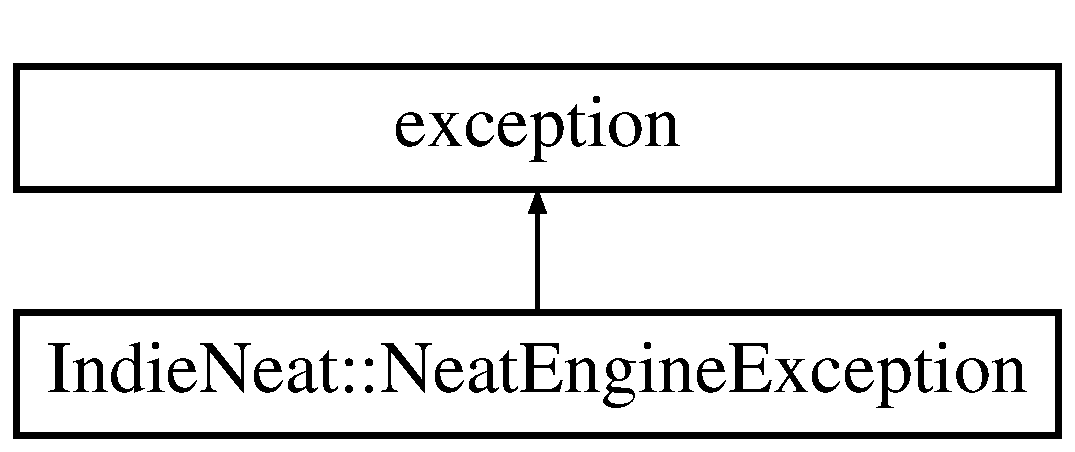
\includegraphics[height=2.000000cm]{class_indie_neat_1_1_neat_engine_exception}
\end{center}
\end{figure}
\subsection*{Public Member Functions}
\begin{DoxyCompactItemize}
\item 
\mbox{\Hypertarget{class_indie_neat_1_1_neat_engine_exception_a47aeecd069e952c8f2a099bdb071de7c}\label{class_indie_neat_1_1_neat_engine_exception_a47aeecd069e952c8f2a099bdb071de7c}} 
{\bfseries Neat\+Engine\+Exception} (std\+::string const \&msg)  throw ()
\item 
\mbox{\Hypertarget{class_indie_neat_1_1_neat_engine_exception_a55ce9805a9033945380d1926ebd4ada4}\label{class_indie_neat_1_1_neat_engine_exception_a55ce9805a9033945380d1926ebd4ada4}} 
{\bfseries Neat\+Engine\+Exception} (\hyperlink{class_indie_neat_1_1_neat_engine_exception}{Neat\+Engine\+Exception} const \&)  throw ()
\item 
\mbox{\Hypertarget{class_indie_neat_1_1_neat_engine_exception_a28dfd2e238c68fc58faaeae3bf13fc54}\label{class_indie_neat_1_1_neat_engine_exception_a28dfd2e238c68fc58faaeae3bf13fc54}} 
\hyperlink{class_indie_neat_1_1_neat_engine_exception}{Neat\+Engine\+Exception} \& {\bfseries operator=} (\hyperlink{class_indie_neat_1_1_neat_engine_exception}{Neat\+Engine\+Exception} const \&)  throw ()
\item 
\mbox{\Hypertarget{class_indie_neat_1_1_neat_engine_exception_a007205e8f089da458f2728708f9d7c4c}\label{class_indie_neat_1_1_neat_engine_exception_a007205e8f089da458f2728708f9d7c4c}} 
const char $\ast$ {\bfseries what} (void) const  throw ()
\end{DoxyCompactItemize}


The documentation for this class was generated from the following files\+:\begin{DoxyCompactItemize}
\item 
src/Neat\+Engine\+Exception.\+hh\item 
src/Neat\+Engine\+Exception.\+cpp\end{DoxyCompactItemize}

\hypertarget{class_neat_pool}{}\section{Neat\+Pool$<$ T, Args $>$ Class Template Reference}
\label{class_neat_pool}\index{Neat\+Pool$<$ T, Args $>$@{Neat\+Pool$<$ T, Args $>$}}
\subsection*{Public Member Functions}
\begin{DoxyCompactItemize}
\item 
\mbox{\Hypertarget{class_neat_pool_a3f05eb4f5c7dcdbc6cc30e63374ca925}\label{class_neat_pool_a3f05eb4f5c7dcdbc6cc30e63374ca925}} 
{\bfseries Neat\+Pool} (unsigned nb\+Elements, Args ... args)
\item 
\mbox{\Hypertarget{class_neat_pool_abaae97ca76236acdd3c2cc4f77da2f62}\label{class_neat_pool_abaae97ca76236acdd3c2cc4f77da2f62}} 
void {\bfseries init} (unsigned nb\+Elements, Args ... args)
\item 
\mbox{\Hypertarget{class_neat_pool_ac787d58e31027eee894a87ad2935a822}\label{class_neat_pool_ac787d58e31027eee894a87ad2935a822}} 
{\footnotesize template$<$unsigned ... idx$>$ }\\void {\bfseries build\+New\+Object} (std\+::integer\+\_\+sequence$<$ unsigned, idx ... $>$)
\item 
\mbox{\Hypertarget{class_neat_pool_a0cc52b8bf46f777543c536ffb321755e}\label{class_neat_pool_a0cc52b8bf46f777543c536ffb321755e}} 
T $\ast$ {\bfseries get} ()
\item 
\mbox{\Hypertarget{class_neat_pool_aa649761480b7c3e605a1c5eba6a2423c}\label{class_neat_pool_aa649761480b7c3e605a1c5eba6a2423c}} 
void {\bfseries operator$>$$>$} (T $\ast$\&dest)
\item 
\mbox{\Hypertarget{class_neat_pool_a517c154eaa25f73f33265622ee4a90af}\label{class_neat_pool_a517c154eaa25f73f33265622ee4a90af}} 
void {\bfseries operator$<$$<$} (T $\ast$water)
\end{DoxyCompactItemize}


The documentation for this class was generated from the following file\+:\begin{DoxyCompactItemize}
\item 
src/Neat\+Pool.\+hpp\end{DoxyCompactItemize}

\hypertarget{class_indie_neat_1_1_genotype_1_1_node}{}\section{Indie\+Neat\+:\+:Genotype$<$ num\+Inputs, num\+Outputs $>$\+:\+:Node Class Reference}
\label{class_indie_neat_1_1_genotype_1_1_node}\index{Indie\+Neat\+::\+Genotype$<$ num\+Inputs, num\+Outputs $>$\+::\+Node@{Indie\+Neat\+::\+Genotype$<$ num\+Inputs, num\+Outputs $>$\+::\+Node}}
\subsection*{Public Member Functions}
\begin{DoxyCompactItemize}
\item 
\mbox{\Hypertarget{class_indie_neat_1_1_genotype_1_1_node_a5d7418b3e1291d81039bb52ad13225c7}\label{class_indie_neat_1_1_genotype_1_1_node_a5d7418b3e1291d81039bb52ad13225c7}} 
{\bfseries Node} (unsigned int id, Node\+Type type, double bias)
\item 
\mbox{\Hypertarget{class_indie_neat_1_1_genotype_1_1_node_ac0e4a7684c7cf3a528aa106298b00a14}\label{class_indie_neat_1_1_genotype_1_1_node_ac0e4a7684c7cf3a528aa106298b00a14}} 
{\bfseries Node} (\hyperlink{class_indie_neat_1_1_genotype_1_1_node}{Node} const \&copy)
\item 
\mbox{\Hypertarget{class_indie_neat_1_1_genotype_1_1_node_a65051b7669a59c4c4568e71592e92ef1}\label{class_indie_neat_1_1_genotype_1_1_node_a65051b7669a59c4c4568e71592e92ef1}} 
\hyperlink{class_indie_neat_1_1_genotype_1_1_node}{Node} \& {\bfseries operator=} (\hyperlink{class_indie_neat_1_1_genotype_1_1_node}{Node} const \&copy)
\item 
\mbox{\Hypertarget{class_indie_neat_1_1_genotype_1_1_node_a3951e1029ba41ae1b584b0f374ef91ec}\label{class_indie_neat_1_1_genotype_1_1_node_a3951e1029ba41ae1b584b0f374ef91ec}} 
unsigned int {\bfseries Id} (void) const
\item 
\mbox{\Hypertarget{class_indie_neat_1_1_genotype_1_1_node_a1fde22ec1338f9fbe03a18cdb4052d41}\label{class_indie_neat_1_1_genotype_1_1_node_a1fde22ec1338f9fbe03a18cdb4052d41}} 
unsigned int \& {\bfseries Id} (void)
\item 
\mbox{\Hypertarget{class_indie_neat_1_1_genotype_1_1_node_ac93e7a4380f8a758a645c96ecbf24b4e}\label{class_indie_neat_1_1_genotype_1_1_node_ac93e7a4380f8a758a645c96ecbf24b4e}} 
Node\+Type {\bfseries Type} (void) const
\item 
\mbox{\Hypertarget{class_indie_neat_1_1_genotype_1_1_node_a342408de90a77b653ac7b8321486ddf1}\label{class_indie_neat_1_1_genotype_1_1_node_a342408de90a77b653ac7b8321486ddf1}} 
Node\+Type \& {\bfseries Type} (void)
\item 
\mbox{\Hypertarget{class_indie_neat_1_1_genotype_1_1_node_a0071ac8dda692f16c518d4446da9a257}\label{class_indie_neat_1_1_genotype_1_1_node_a0071ac8dda692f16c518d4446da9a257}} 
double {\bfseries Bias} (void) const
\item 
\mbox{\Hypertarget{class_indie_neat_1_1_genotype_1_1_node_ae31fd0bcb4e8296ef7b184ff3b5889ba}\label{class_indie_neat_1_1_genotype_1_1_node_ae31fd0bcb4e8296ef7b184ff3b5889ba}} 
double \& {\bfseries Bias} (void)
\end{DoxyCompactItemize}


The documentation for this class was generated from the following file\+:\begin{DoxyCompactItemize}
\item 
src/Genotype.\+hpp\end{DoxyCompactItemize}

\hypertarget{class_indie_neat_1_1_operator}{}\section{Indie\+Neat\+:\+:Operator$<$ num\+Inputs, num\+Outputs $>$ Class Template Reference}
\label{class_indie_neat_1_1_operator}\index{Indie\+Neat\+::\+Operator$<$ num\+Inputs, num\+Outputs $>$@{Indie\+Neat\+::\+Operator$<$ num\+Inputs, num\+Outputs $>$}}
\subsection*{Classes}
\begin{DoxyCompactItemize}
\item 
struct \hyperlink{struct_indie_neat_1_1_operator_1_1_settings}{Settings}
\end{DoxyCompactItemize}
\subsection*{Static Public Member Functions}
\begin{DoxyCompactItemize}
\item 
\mbox{\Hypertarget{class_indie_neat_1_1_operator_a3906c464cb3fe586ac8d0cbdcb8d57a8}\label{class_indie_neat_1_1_operator_a3906c464cb3fe586ac8d0cbdcb8d57a8}} 
static void {\bfseries Set} (\hyperlink{struct_indie_neat_1_1_operator_1_1_settings}{Settings} const \&)
\item 
\mbox{\Hypertarget{class_indie_neat_1_1_operator_ad509f15148687f615db47089c89040a7}\label{class_indie_neat_1_1_operator_ad509f15148687f615db47089c89040a7}} 
static void {\bfseries Line\+Up} (std\+::vector$<$ typename \hyperlink{class_indie_neat_1_1_genotype}{Genotype}$<$ num\+Inputs, num\+Outputs $>$\+::Gene $\ast$$>$ const \&g1, std\+::vector$<$ typename \hyperlink{class_indie_neat_1_1_genotype}{Genotype}$<$ num\+Inputs, num\+Outputs $>$\+::Gene $\ast$$>$ const \&g2, std\+::vector$<$ typename \hyperlink{class_indie_neat_1_1_genotype}{Genotype}$<$ num\+Inputs, num\+Outputs $>$\+::Gene $\ast$$>$ \&p1, std\+::vector$<$ typename \hyperlink{class_indie_neat_1_1_genotype}{Genotype}$<$ num\+Inputs, num\+Outputs $>$\+::Gene $\ast$$>$ \&p2)
\item 
\mbox{\Hypertarget{class_indie_neat_1_1_operator_a82837d3db032d7817d0a09ef6616d88c}\label{class_indie_neat_1_1_operator_a82837d3db032d7817d0a09ef6616d88c}} 
static \hyperlink{class_indie_neat_1_1_genotype}{Genotype}$<$ num\+Inputs, num\+Outputs $>$ $\ast$ {\bfseries Crossover} (\hyperlink{class_indie_neat_1_1_genotype}{Genotype}$<$ num\+Inputs, num\+Outputs $>$ const \&g1, \hyperlink{class_indie_neat_1_1_genotype}{Genotype}$<$ num\+Inputs, num\+Outputs $>$ const \&g2)
\item 
\mbox{\Hypertarget{class_indie_neat_1_1_operator_a1d919a95458ce37d7be2b0231785d4dd}\label{class_indie_neat_1_1_operator_a1d919a95458ce37d7be2b0231785d4dd}} 
static double {\bfseries Compute\+Distance} (\hyperlink{class_indie_neat_1_1_genotype}{Genotype}$<$ num\+Inputs, num\+Outputs $>$ const \&g1, \hyperlink{class_indie_neat_1_1_genotype}{Genotype}$<$ num\+Inputs, num\+Outputs $>$ const \&g2, unsigned int max\+Genome\+Size)
\end{DoxyCompactItemize}


The documentation for this class was generated from the following file\+:\begin{DoxyCompactItemize}
\item 
src/Operator.\+hpp\end{DoxyCompactItemize}

\hypertarget{struct_indie_neat_1_1_backup_1_1_packed_genome}{}\section{Indie\+Neat\+:\+:Backup$<$ num\+Inputs, num\+Outputs $>$\+:\+:Packed\+Genome Struct Reference}
\label{struct_indie_neat_1_1_backup_1_1_packed_genome}\index{Indie\+Neat\+::\+Backup$<$ num\+Inputs, num\+Outputs $>$\+::\+Packed\+Genome@{Indie\+Neat\+::\+Backup$<$ num\+Inputs, num\+Outputs $>$\+::\+Packed\+Genome}}
\subsection*{Public Attributes}
\begin{DoxyCompactItemize}
\item 
\mbox{\Hypertarget{struct_indie_neat_1_1_backup_1_1_packed_genome_a8fe278f6fa33061fc8c3bdf0484d582e}\label{struct_indie_neat_1_1_backup_1_1_packed_genome_a8fe278f6fa33061fc8c3bdf0484d582e}} 
long long {\bfseries num\+Nodes}
\item 
\mbox{\Hypertarget{struct_indie_neat_1_1_backup_1_1_packed_genome_a4ccbe78013e1121f62e5f04cf3fc0273}\label{struct_indie_neat_1_1_backup_1_1_packed_genome_a4ccbe78013e1121f62e5f04cf3fc0273}} 
double {\bfseries fitness}
\item 
\mbox{\Hypertarget{struct_indie_neat_1_1_backup_1_1_packed_genome_a540728e0e897a51437f79eea85cf9d95}\label{struct_indie_neat_1_1_backup_1_1_packed_genome_a540728e0e897a51437f79eea85cf9d95}} 
std\+::vector$<$ typename \hyperlink{class_indie_neat_1_1_genotype}{Genotype}$<$ num\+Inputs, num\+Outputs $>$\+::Node $\ast$ $>$ {\bfseries nodes}
\item 
\mbox{\Hypertarget{struct_indie_neat_1_1_backup_1_1_packed_genome_ad5bb9e15c7c9a81b2acc466e9434a4c2}\label{struct_indie_neat_1_1_backup_1_1_packed_genome_ad5bb9e15c7c9a81b2acc466e9434a4c2}} 
std\+::vector$<$ typename \hyperlink{class_indie_neat_1_1_genotype}{Genotype}$<$ num\+Inputs, num\+Outputs $>$\+::Gene $\ast$ $>$ {\bfseries genes}
\end{DoxyCompactItemize}


The documentation for this struct was generated from the following file\+:\begin{DoxyCompactItemize}
\item 
src/Backup.\+hpp\end{DoxyCompactItemize}

\hypertarget{struct_indie_neat_1_1_backup_1_1_params}{}\section{Indie\+Neat\+:\+:Backup$<$ num\+Inputs, num\+Outputs $>$\+:\+:Params Struct Reference}
\label{struct_indie_neat_1_1_backup_1_1_params}\index{Indie\+Neat\+::\+Backup$<$ num\+Inputs, num\+Outputs $>$\+::\+Params@{Indie\+Neat\+::\+Backup$<$ num\+Inputs, num\+Outputs $>$\+::\+Params}}
\subsection*{Public Attributes}
\begin{DoxyCompactItemize}
\item 
\mbox{\Hypertarget{struct_indie_neat_1_1_backup_1_1_params_acbbb31260ac7ee6aa67c7b4ea5ece152}\label{struct_indie_neat_1_1_backup_1_1_params_acbbb31260ac7ee6aa67c7b4ea5ece152}} 
unsigned int {\bfseries Population\+Size}
\item 
\mbox{\Hypertarget{struct_indie_neat_1_1_backup_1_1_params_a58878b4923e2812f1679f1ad1fa3b6b6}\label{struct_indie_neat_1_1_backup_1_1_params_a58878b4923e2812f1679f1ad1fa3b6b6}} 
unsigned int {\bfseries Max\+Stagnant\+Generation}
\item 
\mbox{\Hypertarget{struct_indie_neat_1_1_backup_1_1_params_a87cbf2c1e1bdd474f6198893b9513493}\label{struct_indie_neat_1_1_backup_1_1_params_a87cbf2c1e1bdd474f6198893b9513493}} 
double {\bfseries Distance\+Threshold}
\item 
\mbox{\Hypertarget{struct_indie_neat_1_1_backup_1_1_params_a43b2e1fed098168ba66e9e495b20c8a4}\label{struct_indie_neat_1_1_backup_1_1_params_a43b2e1fed098168ba66e9e495b20c8a4}} 
double {\bfseries Offsprings\+Rate}
\item 
\mbox{\Hypertarget{struct_indie_neat_1_1_backup_1_1_params_a6f31baa5e334ad02bc9f715a4b2571b3}\label{struct_indie_neat_1_1_backup_1_1_params_a6f31baa5e334ad02bc9f715a4b2571b3}} 
double {\bfseries Inter\+Species\+Mating\+Rate}
\item 
\mbox{\Hypertarget{struct_indie_neat_1_1_backup_1_1_params_ad2b4ade3e850705f933290403412529a}\label{struct_indie_neat_1_1_backup_1_1_params_ad2b4ade3e850705f933290403412529a}} 
double {\bfseries Species\+Keeping\+Rate}
\item 
\mbox{\Hypertarget{struct_indie_neat_1_1_backup_1_1_params_a7a4f488dba9eee908013d641f0a51ee8}\label{struct_indie_neat_1_1_backup_1_1_params_a7a4f488dba9eee908013d641f0a51ee8}} 
unsigned int {\bfseries Default\+Species\+Pool\+Size}
\item 
\mbox{\Hypertarget{struct_indie_neat_1_1_backup_1_1_params_a67d9292ea9e640a5729fe5d631685089}\label{struct_indie_neat_1_1_backup_1_1_params_a67d9292ea9e640a5729fe5d631685089}} 
std\+::pair$<$ double, double $>$ {\bfseries Default\+Weight\+Range}
\item 
\mbox{\Hypertarget{struct_indie_neat_1_1_backup_1_1_params_a1e6a5e73cbc492081f36b0896e9bf093}\label{struct_indie_neat_1_1_backup_1_1_params_a1e6a5e73cbc492081f36b0896e9bf093}} 
double {\bfseries Excess\+Coeficient}
\item 
\mbox{\Hypertarget{struct_indie_neat_1_1_backup_1_1_params_a50e77dabfd18313b2586fe619824f8fe}\label{struct_indie_neat_1_1_backup_1_1_params_a50e77dabfd18313b2586fe619824f8fe}} 
double {\bfseries Disjoint\+Coeficient}
\item 
\mbox{\Hypertarget{struct_indie_neat_1_1_backup_1_1_params_a8215ecb87dd748332639c916f21043c2}\label{struct_indie_neat_1_1_backup_1_1_params_a8215ecb87dd748332639c916f21043c2}} 
double {\bfseries Weight\+Average\+Coeficient}
\item 
\mbox{\Hypertarget{struct_indie_neat_1_1_backup_1_1_params_adf6978ca30f0912f9edaeb84f5c24c0b}\label{struct_indie_neat_1_1_backup_1_1_params_adf6978ca30f0912f9edaeb84f5c24c0b}} 
std\+::pair$<$ double, double $>$ {\bfseries Default\+Perturbation\+Range}
\item 
\mbox{\Hypertarget{struct_indie_neat_1_1_backup_1_1_params_ad0ef3e3b83aad87c007a1fee6953b5b8}\label{struct_indie_neat_1_1_backup_1_1_params_ad0ef3e3b83aad87c007a1fee6953b5b8}} 
double {\bfseries Expected\+Fitness}
\item 
\mbox{\Hypertarget{struct_indie_neat_1_1_backup_1_1_params_af96da1ac4c8da9d7899e92bfb67b6591}\label{struct_indie_neat_1_1_backup_1_1_params_af96da1ac4c8da9d7899e92bfb67b6591}} 
unsigned int {\bfseries Maximum\+Generation}
\item 
\mbox{\Hypertarget{struct_indie_neat_1_1_backup_1_1_params_a2a0881115e1ea4485bc2f4b5d9898174}\label{struct_indie_neat_1_1_backup_1_1_params_a2a0881115e1ea4485bc2f4b5d9898174}} 
double {\bfseries Add\+Neuron\+Probability}
\item 
\mbox{\Hypertarget{struct_indie_neat_1_1_backup_1_1_params_ab0af28fee860496a83b56597dc4dac1d}\label{struct_indie_neat_1_1_backup_1_1_params_ab0af28fee860496a83b56597dc4dac1d}} 
double {\bfseries Add\+Connection\+Probability}
\item 
\mbox{\Hypertarget{struct_indie_neat_1_1_backup_1_1_params_a93e861ef6f03ce10b529c377eb832ec5}\label{struct_indie_neat_1_1_backup_1_1_params_a93e861ef6f03ce10b529c377eb832ec5}} 
double {\bfseries Random\+Weight\+Probability}
\end{DoxyCompactItemize}


The documentation for this struct was generated from the following file\+:\begin{DoxyCompactItemize}
\item 
src/Backup.\+hpp\end{DoxyCompactItemize}

\hypertarget{class_indie_neat_1_1_phenotype}{}\section{Indie\+Neat\+:\+:Phenotype$<$ num\+Inputs, num\+Outputs $>$ Class Template Reference}
\label{class_indie_neat_1_1_phenotype}\index{Indie\+Neat\+::\+Phenotype$<$ num\+Inputs, num\+Outputs $>$@{Indie\+Neat\+::\+Phenotype$<$ num\+Inputs, num\+Outputs $>$}}


Allows to interpret \hyperlink{class_indie_neat_1_1_genotype}{Genotype} into \hyperlink{class_indie_neat_1_1_phenotype}{Phenotype}.  




{\ttfamily \#include $<$Phenotype.\+hpp$>$}

\subsection*{Public Member Functions}
\begin{DoxyCompactItemize}
\item 
\hyperlink{class_indie_neat_1_1_phenotype_a073fe9386602c8cce9dac9fc78bbce35}{Phenotype} (\hyperlink{class_indie_neat_1_1_genotype}{Genotype}$<$ num\+Inputs, num\+Outputs $>$ const \&genome)
\begin{DoxyCompactList}\small\item\em Construct a phenotype with a given genome. \end{DoxyCompactList}\item 
\mbox{\Hypertarget{class_indie_neat_1_1_phenotype_a68ce3283f94cda0581322ba4fcf10ae8}\label{class_indie_neat_1_1_phenotype_a68ce3283f94cda0581322ba4fcf10ae8}} 
\hyperlink{class_indie_neat_1_1_phenotype_a68ce3283f94cda0581322ba4fcf10ae8}{$\sim$\+Phenotype} (void)
\begin{DoxyCompactList}\small\item\em Destructor of \hyperlink{class_indie_neat_1_1_phenotype}{Phenotype} class. Destructor of \hyperlink{class_indie_neat_1_1_phenotype}{Phenotype} class. \end{DoxyCompactList}\item 
\mbox{\Hypertarget{class_indie_neat_1_1_phenotype_a2a8d1351b2d63539e825fa720ff9699e}\label{class_indie_neat_1_1_phenotype_a2a8d1351b2d63539e825fa720ff9699e}} 
void {\bfseries init} (void)
\item 
\mbox{\Hypertarget{class_indie_neat_1_1_phenotype_acf8ee08e9e881f33ca40f4d839a39a79}\label{class_indie_neat_1_1_phenotype_acf8ee08e9e881f33ca40f4d839a39a79}} 
std\+::vector$<$ double $>$ const  \& {\bfseries get\+Outputs} (void) const
\item 
\mbox{\Hypertarget{class_indie_neat_1_1_phenotype_a8b5049674532efec31c7f4a0b742ec18}\label{class_indie_neat_1_1_phenotype_a8b5049674532efec31c7f4a0b742ec18}} 
std\+::vector$<$ double $>$ const  \& {\bfseries feed\+Forward} (std\+::vector$<$ double $>$ const \&inputs)
\end{DoxyCompactItemize}


\subsection{Detailed Description}
\subsubsection*{template$<$unsigned int num\+Inputs, unsigned int num\+Outputs$>$\newline
class Indie\+Neat\+::\+Phenotype$<$ num\+Inputs, num\+Outputs $>$}

Allows to interpret \hyperlink{class_indie_neat_1_1_genotype}{Genotype} into \hyperlink{class_indie_neat_1_1_phenotype}{Phenotype}. 

With this class, you can create a phenotype based on the given genotype. It will allows you to compute the result of your model in terms of the inputs. 
\begin{DoxyTemplParams}{Template Parameters}
{\em num\+Inputs} & Describe how many input takes the phenotype. \\
\hline
{\em num\+Outputs} & Describe how many outputs has the phenotype. \\
\hline
\end{DoxyTemplParams}


\subsection{Constructor \& Destructor Documentation}
\mbox{\Hypertarget{class_indie_neat_1_1_phenotype_a073fe9386602c8cce9dac9fc78bbce35}\label{class_indie_neat_1_1_phenotype_a073fe9386602c8cce9dac9fc78bbce35}} 
\index{Indie\+Neat\+::\+Phenotype@{Indie\+Neat\+::\+Phenotype}!Phenotype@{Phenotype}}
\index{Phenotype@{Phenotype}!Indie\+Neat\+::\+Phenotype@{Indie\+Neat\+::\+Phenotype}}
\subsubsection{\texorpdfstring{Phenotype()}{Phenotype()}}
{\footnotesize\ttfamily template$<$unsigned int num\+Inputs, unsigned int num\+Outputs$>$ \\
\hyperlink{class_indie_neat_1_1_phenotype}{Indie\+Neat\+::\+Phenotype}$<$ num\+Inputs, num\+Outputs $>$\+::\hyperlink{class_indie_neat_1_1_phenotype}{Phenotype} (\begin{DoxyParamCaption}\item[{\hyperlink{class_indie_neat_1_1_genotype}{Genotype}$<$ num\+Inputs, num\+Outputs $>$ const \&}]{genome }\end{DoxyParamCaption})\hspace{0.3cm}{\ttfamily [inline]}}



Construct a phenotype with a given genome. 

Construct a phenotype based on the given genome. 
\begin{DoxyParams}{Parameters}
{\em genome} & Contains all the information about the genome to construct the phenotype. \\
\hline
\end{DoxyParams}


The documentation for this class was generated from the following file\+:\begin{DoxyCompactItemize}
\item 
src/Phenotype.\+hpp\end{DoxyCompactItemize}

\hypertarget{class_indie_neat_1_1_population}{}\section{Indie\+Neat\+:\+:Population$<$ num\+Inputs, num\+Outputs $>$ Class Template Reference}
\label{class_indie_neat_1_1_population}\index{Indie\+Neat\+::\+Population$<$ num\+Inputs, num\+Outputs $>$@{Indie\+Neat\+::\+Population$<$ num\+Inputs, num\+Outputs $>$}}
\subsection*{Classes}
\begin{DoxyCompactItemize}
\item 
struct \hyperlink{struct_indie_neat_1_1_population_1_1_genome_container}{Genome\+Container}
\item 
struct \hyperlink{struct_indie_neat_1_1_population_1_1_genome_score}{Genome\+Score}
\item 
struct \hyperlink{struct_indie_neat_1_1_population_1_1_settings}{Settings}
\item 
class \hyperlink{class_indie_neat_1_1_population_1_1_species}{Species}
\end{DoxyCompactItemize}
\subsection*{Public Member Functions}
\begin{DoxyCompactItemize}
\item 
\mbox{\Hypertarget{class_indie_neat_1_1_population_ab9c85c50e1476700ad373a8f536e8898}\label{class_indie_neat_1_1_population_ab9c85c50e1476700ad373a8f536e8898}} 
{\bfseries Population} (\hyperlink{struct_indie_neat_1_1_population_1_1_settings}{Settings} const \&settings)
\item 
\mbox{\Hypertarget{class_indie_neat_1_1_population_a32ef3a36f8b74bd4a75981e0d3ec1d2b}\label{class_indie_neat_1_1_population_a32ef3a36f8b74bd4a75981e0d3ec1d2b}} 
{\bfseries Population} (\hyperlink{class_indie_neat_1_1_population}{Population} const \&copy)
\item 
\mbox{\Hypertarget{class_indie_neat_1_1_population_a24b43b8cd8743d15542980e124acb6a5}\label{class_indie_neat_1_1_population_a24b43b8cd8743d15542980e124acb6a5}} 
\hyperlink{class_indie_neat_1_1_population}{Population} \& {\bfseries operator=} (\hyperlink{class_indie_neat_1_1_population}{Population} const \&copy)
\item 
\mbox{\Hypertarget{class_indie_neat_1_1_population_a250935f7589600cd6ed661288c09f760}\label{class_indie_neat_1_1_population_a250935f7589600cd6ed661288c09f760}} 
void {\bfseries init} (\hyperlink{struct_indie_neat_1_1_population_1_1_settings}{Settings} const \&settings)
\item 
\mbox{\Hypertarget{class_indie_neat_1_1_population_ab8d6e15a79aa6138e3c369718a727690}\label{class_indie_neat_1_1_population_ab8d6e15a79aa6138e3c369718a727690}} 
void {\bfseries set\+Settings} (\hyperlink{struct_indie_neat_1_1_population_1_1_settings}{Settings} const \&settings)
\item 
\mbox{\Hypertarget{class_indie_neat_1_1_population_a22efadab423680576c832cf3a575f49a}\label{class_indie_neat_1_1_population_a22efadab423680576c832cf3a575f49a}} 
std\+::vector$<$ \hyperlink{class_indie_neat_1_1_genotype}{Genotype}$<$ num\+Inputs, num\+Outputs $>$ $\ast$ $>$ const  \& {\bfseries Genomes} (void) const
\item 
\mbox{\Hypertarget{class_indie_neat_1_1_population_a721b58835393fd9cb534e7c3838277eb}\label{class_indie_neat_1_1_population_a721b58835393fd9cb534e7c3838277eb}} 
void {\bfseries evaluate} (std\+::vector$<$ \hyperlink{struct_indie_neat_1_1_population_1_1_genome_container}{Genome\+Container} $\ast$$>$ \&buffer, unsigned int num\+Of\+Genomes)
\item 
\mbox{\Hypertarget{class_indie_neat_1_1_population_ae681e4f9a1f67c0b050b35a1b7974444}\label{class_indie_neat_1_1_population_ae681e4f9a1f67c0b050b35a1b7974444}} 
void {\bfseries push\+Score} (std\+::vector$<$ \hyperlink{struct_indie_neat_1_1_population_1_1_genome_score}{Genome\+Score} $\ast$$>$ const \&scores)
\item 
\mbox{\Hypertarget{class_indie_neat_1_1_population_a96eb698db1c2f09a6d202643cdc4ae52}\label{class_indie_neat_1_1_population_a96eb698db1c2f09a6d202643cdc4ae52}} 
double {\bfseries get\+Max\+Fitness} (void) const
\item 
\mbox{\Hypertarget{class_indie_neat_1_1_population_a3a12ba241a847a9357be211f82fef815}\label{class_indie_neat_1_1_population_a3a12ba241a847a9357be211f82fef815}} 
\hyperlink{class_indie_neat_1_1_genotype}{Genotype}$<$ num\+Inputs, num\+Outputs $>$ const  \& {\bfseries get\+Best\+Genome} (void) const
\item 
\mbox{\Hypertarget{class_indie_neat_1_1_population_a579fa4d9fdf0b50b462b54bed3b0a8ec}\label{class_indie_neat_1_1_population_a579fa4d9fdf0b50b462b54bed3b0a8ec}} 
bool {\bfseries is\+Evolving} (void) const
\item 
\mbox{\Hypertarget{class_indie_neat_1_1_population_ad176c408329efa7387880de7d1c2d540}\label{class_indie_neat_1_1_population_ad176c408329efa7387880de7d1c2d540}} 
bool {\bfseries is\+Finished} (void) const
\item 
\mbox{\Hypertarget{class_indie_neat_1_1_population_a46d92dda9ad0a6e499783da8e40ccc97}\label{class_indie_neat_1_1_population_a46d92dda9ad0a6e499783da8e40ccc97}} 
bool {\bfseries save} (void) const
\item 
\mbox{\Hypertarget{class_indie_neat_1_1_population_a407e6e0437e79aaa4483cdd3cf4cb3a0}\label{class_indie_neat_1_1_population_a407e6e0437e79aaa4483cdd3cf4cb3a0}} 
bool {\bfseries load} (std\+::string const \&dirname)
\end{DoxyCompactItemize}


The documentation for this class was generated from the following file\+:\begin{DoxyCompactItemize}
\item 
src/Population.\+hpp\end{DoxyCompactItemize}

\hypertarget{struct_indie_neat_1_1_population_1_1_settings}{}\section{Indie\+Neat\+:\+:Population$<$ num\+Inputs, num\+Outputs $>$\+:\+:Settings Struct Reference}
\label{struct_indie_neat_1_1_population_1_1_settings}\index{Indie\+Neat\+::\+Population$<$ num\+Inputs, num\+Outputs $>$\+::\+Settings@{Indie\+Neat\+::\+Population$<$ num\+Inputs, num\+Outputs $>$\+::\+Settings}}
\subsection*{Public Member Functions}
\begin{DoxyCompactItemize}
\item 
\mbox{\Hypertarget{struct_indie_neat_1_1_population_1_1_settings_ac2defa65f2152b868393d7a17e140f8c}\label{struct_indie_neat_1_1_population_1_1_settings_ac2defa65f2152b868393d7a17e140f8c}} 
{\bfseries Settings} (\hyperlink{struct_indie_neat_1_1_population_1_1_settings}{Settings} const \&copy)
\item 
\mbox{\Hypertarget{struct_indie_neat_1_1_population_1_1_settings_ad384b6f77208d8afd9bb360ee626e57a}\label{struct_indie_neat_1_1_population_1_1_settings_ad384b6f77208d8afd9bb360ee626e57a}} 
\hyperlink{struct_indie_neat_1_1_population_1_1_settings}{Settings} \& {\bfseries operator=} (\hyperlink{struct_indie_neat_1_1_population_1_1_settings}{Settings} const \&copy)
\end{DoxyCompactItemize}
\subsection*{Public Attributes}
\begin{DoxyCompactItemize}
\item 
\mbox{\Hypertarget{struct_indie_neat_1_1_population_1_1_settings_a14aafe30a58b2689a13dd1d19500a18f}\label{struct_indie_neat_1_1_population_1_1_settings_a14aafe30a58b2689a13dd1d19500a18f}} 
unsigned int {\bfseries population\+Size}
\item 
\mbox{\Hypertarget{struct_indie_neat_1_1_population_1_1_settings_ae6c5b61c539cd4e5dc043f798aa65760}\label{struct_indie_neat_1_1_population_1_1_settings_ae6c5b61c539cd4e5dc043f798aa65760}} 
double {\bfseries distance\+Threshold}
\item 
\mbox{\Hypertarget{struct_indie_neat_1_1_population_1_1_settings_a1004cb5c55fde301f09f8bd74cdebc8c}\label{struct_indie_neat_1_1_population_1_1_settings_a1004cb5c55fde301f09f8bd74cdebc8c}} 
unsigned int {\bfseries stagnant\+Generation\+Number}
\item 
\mbox{\Hypertarget{struct_indie_neat_1_1_population_1_1_settings_ab524a3e59b527c2a3ed587e2e4a71c0e}\label{struct_indie_neat_1_1_population_1_1_settings_ab524a3e59b527c2a3ed587e2e4a71c0e}} 
double {\bfseries offsprings\+Rate}
\item 
\mbox{\Hypertarget{struct_indie_neat_1_1_population_1_1_settings_a5cd70811c28d92d8e7ca7abb1478dab4}\label{struct_indie_neat_1_1_population_1_1_settings_a5cd70811c28d92d8e7ca7abb1478dab4}} 
double {\bfseries inter\+Species\+Mating\+Rate}
\item 
\mbox{\Hypertarget{struct_indie_neat_1_1_population_1_1_settings_a2718afab60e531784caf63603165d24b}\label{struct_indie_neat_1_1_population_1_1_settings_a2718afab60e531784caf63603165d24b}} 
double {\bfseries species\+Keeping\+Rate}
\item 
\mbox{\Hypertarget{struct_indie_neat_1_1_population_1_1_settings_ac23151beeabfcd56f270b8773aae8eae}\label{struct_indie_neat_1_1_population_1_1_settings_ac23151beeabfcd56f270b8773aae8eae}} 
unsigned int {\bfseries default\+Pool\+Size}
\item 
\mbox{\Hypertarget{struct_indie_neat_1_1_population_1_1_settings_a6b5240ac30a735d78ec28547515f0cde}\label{struct_indie_neat_1_1_population_1_1_settings_a6b5240ac30a735d78ec28547515f0cde}} 
std\+::pair$<$ double, double $>$ {\bfseries weight\+Range}
\item 
\mbox{\Hypertarget{struct_indie_neat_1_1_population_1_1_settings_a99d7e84d07d5bc1b8c5974558cb7a22d}\label{struct_indie_neat_1_1_population_1_1_settings_a99d7e84d07d5bc1b8c5974558cb7a22d}} 
double {\bfseries expected\+Fitness}
\item 
\mbox{\Hypertarget{struct_indie_neat_1_1_population_1_1_settings_ad82badf3e35c9aaf91bd12a491a4e528}\label{struct_indie_neat_1_1_population_1_1_settings_ad82badf3e35c9aaf91bd12a491a4e528}} 
unsigned int {\bfseries max\+Generation}
\end{DoxyCompactItemize}


The documentation for this struct was generated from the following file\+:\begin{DoxyCompactItemize}
\item 
src/Population.\+hpp\end{DoxyCompactItemize}

\hypertarget{struct_indie_neat_1_1_operator_1_1_settings}{}\section{Indie\+Neat\+:\+:Operator$<$ num\+Inputs, num\+Outputs $>$\+:\+:Settings Struct Reference}
\label{struct_indie_neat_1_1_operator_1_1_settings}\index{Indie\+Neat\+::\+Operator$<$ num\+Inputs, num\+Outputs $>$\+::\+Settings@{Indie\+Neat\+::\+Operator$<$ num\+Inputs, num\+Outputs $>$\+::\+Settings}}
\subsection*{Public Member Functions}
\begin{DoxyCompactItemize}
\item 
\mbox{\Hypertarget{struct_indie_neat_1_1_operator_1_1_settings_abae993de1b2199df3dcaa49788e8b804}\label{struct_indie_neat_1_1_operator_1_1_settings_abae993de1b2199df3dcaa49788e8b804}} 
{\bfseries Settings} (\hyperlink{struct_indie_neat_1_1_operator_1_1_settings}{Settings} const \&copy)
\item 
\mbox{\Hypertarget{struct_indie_neat_1_1_operator_1_1_settings_a7e2a44df551648c656a6fdcac83a3d75}\label{struct_indie_neat_1_1_operator_1_1_settings_a7e2a44df551648c656a6fdcac83a3d75}} 
\hyperlink{struct_indie_neat_1_1_operator_1_1_settings}{Settings} \& {\bfseries operator=} (\hyperlink{struct_indie_neat_1_1_operator_1_1_settings}{Settings} const \&copy)
\end{DoxyCompactItemize}
\subsection*{Public Attributes}
\begin{DoxyCompactItemize}
\item 
\mbox{\Hypertarget{struct_indie_neat_1_1_operator_1_1_settings_aeed191109e68d20a2a426de8aaae8549}\label{struct_indie_neat_1_1_operator_1_1_settings_aeed191109e68d20a2a426de8aaae8549}} 
std\+::pair$<$ double, double $>$ {\bfseries weight\+Range}
\item 
\mbox{\Hypertarget{struct_indie_neat_1_1_operator_1_1_settings_ade01531239ad56b984fc1ba296965d07}\label{struct_indie_neat_1_1_operator_1_1_settings_ade01531239ad56b984fc1ba296965d07}} 
double {\bfseries excess\+Coef}
\item 
\mbox{\Hypertarget{struct_indie_neat_1_1_operator_1_1_settings_a9bdd3801df3323d02268bffc4fd03b90}\label{struct_indie_neat_1_1_operator_1_1_settings_a9bdd3801df3323d02268bffc4fd03b90}} 
double {\bfseries disjoint\+Coef}
\item 
\mbox{\Hypertarget{struct_indie_neat_1_1_operator_1_1_settings_a7fb0853b84e3c7ff412f28b027918c48}\label{struct_indie_neat_1_1_operator_1_1_settings_a7fb0853b84e3c7ff412f28b027918c48}} 
double {\bfseries weights\+Avg\+Coef}
\end{DoxyCompactItemize}


The documentation for this struct was generated from the following file\+:\begin{DoxyCompactItemize}
\item 
src/Operator.\+hpp\end{DoxyCompactItemize}

\hypertarget{struct_indie_neat_1_1_mutator_1_1_settings}{}\section{Indie\+Neat\+:\+:Mutator$<$ num\+Inputs, num\+Outputs $>$\+:\+:Settings Struct Reference}
\label{struct_indie_neat_1_1_mutator_1_1_settings}\index{Indie\+Neat\+::\+Mutator$<$ num\+Inputs, num\+Outputs $>$\+::\+Settings@{Indie\+Neat\+::\+Mutator$<$ num\+Inputs, num\+Outputs $>$\+::\+Settings}}
\subsection*{Public Member Functions}
\begin{DoxyCompactItemize}
\item 
\mbox{\Hypertarget{struct_indie_neat_1_1_mutator_1_1_settings_aaed707005142f94c0707245196d94807}\label{struct_indie_neat_1_1_mutator_1_1_settings_aaed707005142f94c0707245196d94807}} 
{\bfseries Settings} (std\+::pair$<$ double, double $>$ const \&weightR, std\+::pair$<$ double, double $>$ const \&pertub\+Range, double weightP, double connectionP, double nodeP, double weight\+Mut\+Prob)
\item 
\mbox{\Hypertarget{struct_indie_neat_1_1_mutator_1_1_settings_a85e9e4c7eee813840efa5342147e623f}\label{struct_indie_neat_1_1_mutator_1_1_settings_a85e9e4c7eee813840efa5342147e623f}} 
{\bfseries Settings} (\hyperlink{struct_indie_neat_1_1_mutator_1_1_settings}{Settings} const \&settings)
\item 
\mbox{\Hypertarget{struct_indie_neat_1_1_mutator_1_1_settings_abda6fa8e9a3e2b7b4721610b9d85b04d}\label{struct_indie_neat_1_1_mutator_1_1_settings_abda6fa8e9a3e2b7b4721610b9d85b04d}} 
\hyperlink{struct_indie_neat_1_1_mutator_1_1_settings}{Settings} \& {\bfseries operator=} (\hyperlink{struct_indie_neat_1_1_mutator_1_1_settings}{Settings} const \&settings)
\end{DoxyCompactItemize}
\subsection*{Public Attributes}
\begin{DoxyCompactItemize}
\item 
\mbox{\Hypertarget{struct_indie_neat_1_1_mutator_1_1_settings_ae30aec8ccc7dcfc2a661a7ec36bb5765}\label{struct_indie_neat_1_1_mutator_1_1_settings_ae30aec8ccc7dcfc2a661a7ec36bb5765}} 
std\+::pair$<$ double, double $>$ {\bfseries weight\+Range}
\item 
\mbox{\Hypertarget{struct_indie_neat_1_1_mutator_1_1_settings_a78f388242170815faa91a597d89fcf58}\label{struct_indie_neat_1_1_mutator_1_1_settings_a78f388242170815faa91a597d89fcf58}} 
std\+::pair$<$ double, double $>$ {\bfseries pertubation\+Range}
\item 
\mbox{\Hypertarget{struct_indie_neat_1_1_mutator_1_1_settings_a2bc1c3afedcb9f9235836d4a70e25de2}\label{struct_indie_neat_1_1_mutator_1_1_settings_a2bc1c3afedcb9f9235836d4a70e25de2}} 
double {\bfseries weight\+Rand\+Prob}
\item 
\mbox{\Hypertarget{struct_indie_neat_1_1_mutator_1_1_settings_ad62edb975c3d76c0215a69438f0bcbc7}\label{struct_indie_neat_1_1_mutator_1_1_settings_ad62edb975c3d76c0215a69438f0bcbc7}} 
double {\bfseries add\+Connection\+Prob}
\item 
\mbox{\Hypertarget{struct_indie_neat_1_1_mutator_1_1_settings_a349a029ab408d4e24495eb38b3800f09}\label{struct_indie_neat_1_1_mutator_1_1_settings_a349a029ab408d4e24495eb38b3800f09}} 
double {\bfseries add\+Node\+Prob}
\item 
\mbox{\Hypertarget{struct_indie_neat_1_1_mutator_1_1_settings_ad51d060e7306b4bd09feac87f738219a}\label{struct_indie_neat_1_1_mutator_1_1_settings_ad51d060e7306b4bd09feac87f738219a}} 
double {\bfseries weight\+Mutation\+Prob}
\end{DoxyCompactItemize}


The documentation for this struct was generated from the following file\+:\begin{DoxyCompactItemize}
\item 
src/Mutator.\+hpp\end{DoxyCompactItemize}

\hypertarget{class_indie_neat_1_1_population_1_1_species}{}\section{Indie\+Neat\+:\+:Population$<$ num\+Inputs, num\+Outputs $>$\+:\+:Species Class Reference}
\label{class_indie_neat_1_1_population_1_1_species}\index{Indie\+Neat\+::\+Population$<$ num\+Inputs, num\+Outputs $>$\+::\+Species@{Indie\+Neat\+::\+Population$<$ num\+Inputs, num\+Outputs $>$\+::\+Species}}
\subsection*{Public Member Functions}
\begin{DoxyCompactItemize}
\item 
\mbox{\Hypertarget{class_indie_neat_1_1_population_1_1_species_a87fcfdfb63a564672b8394470f674982}\label{class_indie_neat_1_1_population_1_1_species_a87fcfdfb63a564672b8394470f674982}} 
{\bfseries Species} (\hyperlink{class_indie_neat_1_1_population_1_1_species}{Species} const \&copy)
\item 
\mbox{\Hypertarget{class_indie_neat_1_1_population_1_1_species_ad3529760d9ef0f297b10848bee5dd82e}\label{class_indie_neat_1_1_population_1_1_species_ad3529760d9ef0f297b10848bee5dd82e}} 
\hyperlink{class_indie_neat_1_1_population_1_1_species}{Species} \& {\bfseries operator=} (\hyperlink{class_indie_neat_1_1_population_1_1_species}{Species} const \&copy)
\item 
\mbox{\Hypertarget{class_indie_neat_1_1_population_1_1_species_a927a6e3fbcadf1fd8dc70e0572f45397}\label{class_indie_neat_1_1_population_1_1_species_a927a6e3fbcadf1fd8dc70e0572f45397}} 
void {\bfseries init} (\hyperlink{class_indie_neat_1_1_genotype}{Genotype}$<$ num\+Inputs, num\+Outputs $>$ \&genome)
\item 
\mbox{\Hypertarget{class_indie_neat_1_1_population_1_1_species_ad6237428aa0d689398451c6eed27058c}\label{class_indie_neat_1_1_population_1_1_species_ad6237428aa0d689398451c6eed27058c}} 
void {\bfseries destroy} (void)
\item 
\mbox{\Hypertarget{class_indie_neat_1_1_population_1_1_species_addd4db6f02889048d78cb230bc6be9e7}\label{class_indie_neat_1_1_population_1_1_species_addd4db6f02889048d78cb230bc6be9e7}} 
std\+::vector$<$ \hyperlink{class_indie_neat_1_1_genotype}{Genotype}$<$ num\+Inputs, num\+Outputs $>$ $\ast$ $>$ \& {\bfseries Genomes} (void)
\item 
\mbox{\Hypertarget{class_indie_neat_1_1_population_1_1_species_a98fafc1451a505d95963e0dc2f4555f8}\label{class_indie_neat_1_1_population_1_1_species_a98fafc1451a505d95963e0dc2f4555f8}} 
\hyperlink{class_indie_neat_1_1_genotype}{Genotype}$<$ num\+Inputs, num\+Outputs $>$ \& {\bfseries Reference} (void)
\item 
\mbox{\Hypertarget{class_indie_neat_1_1_population_1_1_species_a51a1a704e3ba31f6b58cbc0e042c404a}\label{class_indie_neat_1_1_population_1_1_species_a51a1a704e3ba31f6b58cbc0e042c404a}} 
void {\bfseries adjust\+Fitness} (double distance\+Threshold, unsigned int max\+Genome\+Size)
\item 
\mbox{\Hypertarget{class_indie_neat_1_1_population_1_1_species_a4569503da7966e73bcefaf19b08ca1b9}\label{class_indie_neat_1_1_population_1_1_species_a4569503da7966e73bcefaf19b08ca1b9}} 
unsigned int {\bfseries number\+Of\+Not\+Evaluated} (void) const
\item 
\mbox{\Hypertarget{class_indie_neat_1_1_population_1_1_species_a7deb0c402c6876ed15e3c8d07d7a458c}\label{class_indie_neat_1_1_population_1_1_species_a7deb0c402c6876ed15e3c8d07d7a458c}} 
unsigned int {\bfseries number\+Of\+Evaluated} (void) const
\item 
\mbox{\Hypertarget{class_indie_neat_1_1_population_1_1_species_a24ef0cd279f380c2d7cf74cd5fdb4622}\label{class_indie_neat_1_1_population_1_1_species_a24ef0cd279f380c2d7cf74cd5fdb4622}} 
\hyperlink{class_indie_neat_1_1_genotype}{Genotype}$<$ num\+Inputs, num\+Outputs $>$ $\ast$ {\bfseries get\+Random\+Genome} (void)
\item 
\mbox{\Hypertarget{class_indie_neat_1_1_population_1_1_species_abd867d0cff4a1f6fd8c2c5dd93cfce0d}\label{class_indie_neat_1_1_population_1_1_species_abd867d0cff4a1f6fd8c2c5dd93cfce0d}} 
void {\bfseries reproduce} (std\+::vector$<$ \hyperlink{class_indie_neat_1_1_genotype}{Genotype}$<$ num\+Inputs, num\+Outputs $>$ $\ast$$>$ \&childs, unsigned int num\+Of\+Childs, double species\+Keeping\+Rate, double inter\+Species\+Mating\+Rate, \hyperlink{class_indie_neat_1_1_population_1_1_species}{Species} \&specie)
\item 
\mbox{\Hypertarget{class_indie_neat_1_1_population_1_1_species_a58d4063013f4370ee63d18e331aa8a95}\label{class_indie_neat_1_1_population_1_1_species_a58d4063013f4370ee63d18e331aa8a95}} 
void {\bfseries evaluate} (std\+::vector$<$ \hyperlink{class_indie_neat_1_1_genotype}{Genotype}$<$ num\+Inputs, num\+Outputs $>$ $\ast$ $>$ \&buffer, unsigned int number\+Of\+Genomes)
\item 
\mbox{\Hypertarget{class_indie_neat_1_1_population_1_1_species_a5119a841f2653f5260d49012a0e25455}\label{class_indie_neat_1_1_population_1_1_species_a5119a841f2653f5260d49012a0e25455}} 
void {\bfseries set\+Stagnant\+Generation} (unsigned int gen)
\item 
\mbox{\Hypertarget{class_indie_neat_1_1_population_1_1_species_a9c3ac1e5c035e05038b6e5e9494207c3}\label{class_indie_neat_1_1_population_1_1_species_a9c3ac1e5c035e05038b6e5e9494207c3}} 
unsigned int {\bfseries get\+Stagnant\+Generation} (void) const
\item 
\mbox{\Hypertarget{class_indie_neat_1_1_population_1_1_species_a894ac24c374fb20f3413642568121a74}\label{class_indie_neat_1_1_population_1_1_species_a894ac24c374fb20f3413642568121a74}} 
double {\bfseries get\+Stagnant\+Fitness} (void) const
\item 
\mbox{\Hypertarget{class_indie_neat_1_1_population_1_1_species_a619f58d475012bc8bce9a52dc3233b43}\label{class_indie_neat_1_1_population_1_1_species_a619f58d475012bc8bce9a52dc3233b43}} 
void {\bfseries set\+Stagnant\+Fitness} (double fit)
\end{DoxyCompactItemize}


The documentation for this class was generated from the following file\+:\begin{DoxyCompactItemize}
\item 
src/Population.\+hpp\end{DoxyCompactItemize}

%--- End generated contents ---

% Index
\backmatter
\newpage
\phantomsection
\clearemptydoublepage
\addcontentsline{toc}{chapter}{Index}
\printindex

\end{document}
